% Khavda: the largest power plant site in the world, and the wires that
% cannot carry it. Beamer deck in the XKDR colour theme.
%
% Build:  ./khavda/build_deck.sh          (pdflatex, twice)
% Notes:  ./khavda/build_deck.sh notes    (presenter notes on a second screen)
%
% Satellite frames come from ./khavda/make_frames.sh (needs Earth Engine
% credentials). Until they exist every satellite slot shows a grey
% placeholder and the deck still compiles.
\documentclass[aspectratio=169,11pt,t]{beamer}

\usepackage[T1]{fontenc}
\usepackage[utf8]{inputenc}
\usepackage[scaled=0.95]{helvet}
\renewcommand{\familydefault}{\sfdefault}
\usepackage{graphicx}
\usepackage{booktabs}
\usepackage{tikz}
\usetikzlibrary{arrows.meta,positioning,calc}
\usepackage{tcolorbox}
\usepackage{animate}
\usepackage{xstring}

% ---- theme -------------------------------------------------------------
\usetheme{default}
\usecolortheme{XKDR}
\usefonttheme{professionalfonts}
\usefonttheme{structurebold}
\setbeamertemplate{navigation symbols}{}
\setbeamertemplate{blocks}[rounded][shadow=false]
\setbeamertemplate{itemize items}{\textcolor{SpOrange}{\rule[0.1ex]{0.9ex}{0.9ex}}}
\setbeamertemplate{enumerate items}[default]
\setbeamercolor{normal text}{fg=SpNearBlack,bg=white}
\setbeamercolor{frametitle}{fg=SpNearBlack,bg=SpLightGray}
\setbeamercolor{item}{fg=SpOrange}
\setbeamercolor{block title}{fg=SpNearBlack,bg=SpLightGray}
\setbeamercolor{block body}{fg=SpNearBlack,bg=SpLightGray!50}
\definecolor{Ink2}{RGB}{90,90,90}
\definecolor{Muted}{RGB}{138,138,138}
\definecolor{Grey}{RGB}{201,201,201}
\setbeamerfont{frametitle}{size=\large,series=\bfseries}
\setbeamerfont{title}{size=\LARGE,series=\bfseries}
\setbeamersize{text margin left=9mm,text margin right=9mm}

% frame title bar: title left, mark right
\setbeamertemplate{frametitle}{%
  \vspace{-1pt}%
  \begin{beamercolorbox}[wd=\paperwidth,ht=10mm,dp=2mm,leftskip=9mm,rightskip=9mm]{frametitle}%
    \usebeamerfont{frametitle}\insertframetitle\hfill
    \raisebox{-1.2mm}{
\includegraphics[height=6mm]{logos/xkdr_mark.png}}%
  \end{beamercolorbox}%
  \vspace{2mm}}

% footline: short title left, page right
\setbeamertemplate{footline}{%
  \begin{beamercolorbox}[wd=\paperwidth,ht=5mm,dp=2.5mm,leftskip=9mm,rightskip=9mm]{normal text}%
    \scriptsize\textcolor{Muted}{Khavda Renewable Energy Park \,\textperiodcentered\, November 2026}%
    \hfill\scriptsize\textcolor{Muted}{\insertframenumber/\inserttotalframenumber}%
  \end{beamercolorbox}}

% ---- satellite frame helpers -------------------------------------------
% frames_meta.tex is written by make_frames.sh: \satLast, \satFirstFile, ...
\providecommand{\satLast}{27}
\providecommand{\satFirstFile}{frames/khavda_00.png}
\providecommand{\satLastFile}{frames/khavda_27.png}
\providecommand{\satGridA}{frames/khavda_00.png}
\providecommand{\satGridB}{frames/khavda_07.png}
\providecommand{\satGridC}{frames/khavda_16.png}
\providecommand{\satGridD}{frames/khavda_22.png}
\providecommand{\satGridE}{frames/khavda_24.png}
\providecommand{\satGridF}{frames/khavda_27.png}
\InputIfFileExists{frames/frames_meta.tex}{}{}
\newif\ifsatframes
\IfFileExists{frames/khavda_00.png}{\satframestrue}{\satframesfalse}

% grey placeholder box: \satplaceholder{width}{caption}
\newcommand{\satplaceholder}[2]{%
  \begin{tikzpicture}
    \node[fill=SpLightGray,draw=Grey,minimum width=#1,minimum height=0.5625*#1,
          text width=0.8*#1,align=center,font=\small\color{Ink2}] {%
      \textbf{Satellite frame not generated yet}\\[2pt]#2\\[4pt]
      \texttt{./khavda/make\_frames.sh}};
  \end{tikzpicture}}

% \satframe{file}{width}{caption shown on the placeholder}
\newcommand{\satframe}[3]{%
  \IfFileExists{#1}{\includegraphics[width=#2]{#1}}{\satplaceholder{#2}{#3}}}

% \satanim{width}: the quarterly animation (1 fps), or the placeholder
\newcommand{\satanim}[1]{%
  \ifsatframes
    \animategraphics[autoplay,loop,width=#1,controls={play,stop}]{1}{frames/khavda_}{00}{\satLast}%
  \else
    \satplaceholder{#1}{The 28-frame quarterly animation, 2020 Q1 to 2026 Q4, one second per frame}%
  \fi}


% title backdrop: the latest frame full-bleed if it exists, else a flat page
\ifsatframes
  \newcommand{\titlebackdrop}{
    \begin{tikzpicture}[remember picture,overlay]
      \node[anchor=center] at (current page.center){\includegraphics[width=\paperwidth]{\satLastFile}};
      \fill[white,opacity=0.86] (current page.south west) rectangle ([yshift=3.6cm]current page.south east);
      \node[anchor=south west,xshift=9mm,yshift=4mm,align=left] at (current page.south west){%
        {\fontsize{28}{32}\selectfont\bfseries\color{SpNearBlack}Khavda}\\[3pt]
        {\large\color{SpNearBlack}The largest power plant site in the world,}\\ {\large\color{SpNearBlack}and the wires that cannot carry it}\\[6pt]
        {\small\color{Ink2}Field briefing \,\textperiodcentered\, November 2026}};
      \node[anchor=south east,xshift=-9mm,yshift=6mm] at (current page.south east){
\includegraphics[width=3.2cm]{logos/xkdr_logo_wide.png}};
    \end{tikzpicture}
}
\else
  \newcommand{\titlebackdrop}{
    \begin{tikzpicture}[remember picture,overlay]
      \fill[SpLightGray] (current page.south west) rectangle (current page.north east);
      \node[anchor=north west,xshift=9mm,yshift=-12mm,align=left] at (current page.north west){%
        {\fontsize{30}{34}\selectfont\bfseries\color{SpNearBlack}Khavda}\\[6pt]
        {\Large\color{SpNearBlack}The largest power plant site in the world,}\\ {\Large\color{SpNearBlack}and the wires that cannot carry it}\\[10pt]
        {\normalsize\color{Ink2}Field briefing \,\textperiodcentered\, November 2026}};
      \node[anchor=south west,xshift=9mm,yshift=9mm,align=left,text width=9cm,font=\footnotesize\color{Ink2}] at (current page.south west)
        {Title background: the latest satellite frame, once \texttt{./khavda/make\_frames.sh} has run.};
      \node[anchor=south east,xshift=-9mm,yshift=9mm] at (current page.south east){
\includegraphics[width=4cm]{logos/xkdr_logo_wide.png}};
    \end{tikzpicture}
}
\fi

\newcommand{\bignum}[2]{{\color{SpOrange}\fontsize{21}{25}\selectfont\textbf{#1}}\\[1pt]{\small\color{Ink2}#2}}
\newcommand{\midnum}[2]{{\color{SpOrange}\fontsize{19}{23}\selectfont\textbf{#1}}\\[1pt]{\footnotesize\color{Ink2}#2}}
\newcommand{\src}[1]{\vfill\hfill{\tiny\color{Muted}#1}}

\title{Khavda}
\subtitle{The largest power plant site in the world, and the wires that cannot carry it}
\author{Field briefing}
\date{November 2026}

\begin{document}

% ==== 1. Title ==========================================================
{\setbeamertemplate{footline}{}
\begin{frame}[plain]
  \titlebackdrop
  \note{Let the picture sit for a moment. It is 726 km², the size of Singapore, and six years ago it was bare salt.}
\end{frame}}

% ==== 2. The animation ====================================================
% The animation is a PDF widget drawn above everything else, so the numbers
% sit beside it rather than over it.
\begin{frame}{Six years in 28 seconds}
  \begin{columns}[T]
    \begin{column}{0.2\textwidth}
      \vspace{1mm}
      {\footnotesize\color{Ink2}One frame a quarter, 2020 to 2026, one second each}\\[6pt]
      \midnum{726 km²}{of salt flat}\\[6pt]
      \midnum{30 GW}{planned}\\[6pt]
      \midnum{14.8 GW}{connected; 9 GW able to leave}
    \end{column}
    \begin{column}{0.8\textwidth}
      \satanim{\textwidth}
    \end{column}
  \end{columns}
  \note{The first four years of frames show roads and camps, not panels. The panels come in 2024 and spread fast. Say that the last number, 9 GW, is the one the rest of the talk explains. The orange outline is the built-up area the software measures in each frame; the hectares are in the legend.}
\end{frame}

% ==== 2b. Six stills ======================================================
\begin{frame}{The same six years in six stills}
  \centering
  \setlength{\tabcolsep}{2pt}
  \begin{tabular}{ccc}
    \satframe{\satGridA}{0.32\textwidth}{2020 Q1: bare salt} &
    \satframe{\satGridB}{0.32\textwidth}{2021 Q4: the approach road} &
    \satframe{\satGridC}{0.32\textwidth}{2024 Q1: first arrays} \\[1pt]
    \satframe{\satGridD}{0.32\textwidth}{2025 Q3: KPS3 opens} &
    \satframe{\satGridE}{0.32\textwidth}{2026 Q1: the 5 GW year} &
    \satframe{\satGridF}{0.32\textwidth}{2026 Q4: latest} \\
  \end{tabular}
  \src{Sentinel-2 cloud-free quarterly composites; contains modified Copernicus Sentinel data. Scene 48 × 27 km centred 24.117° N, 69.350° E.}
  \note{Fallback for viewers that do not play the animation. Top row: land. Bottom row: build. Point at the orange outline growing from the south-west.}
\end{frame}

% ==== 3. Why here =========================================================
\begin{frame}{Why here}
  \begin{columns}[T]
    \begin{column}{0.46\textwidth}
      \vspace{2mm}
      \begin{itemize}\setlength{\itemsep}{6pt}
        \item \textbf{Land nobody lives on.} State wasteland, unsurveyed, no one to buy out.
        \item \textbf{Sun second only to Ladakh.} 2,060 kWh per m² a year, 300 clear days.
        \item \textbf{Wind at 8 metres a second} off the Arabian Sea, strongest at night.
        \item \textbf{One kilometre from Pakistan.} Permits from the Border Security Force, for a site visit too.
      \end{itemize}
    \end{column}
    \begin{column}{0.52\textwidth}
      \satframe{\satFirstFile}{\textwidth}{2020 Q1: the site before construction. White salt crust, the BSF road, India Bridge.}
      {\scriptsize\color{Ink2} The site before building, early 2020. Scale bar lower left.}
    \end{column}
  \end{columns}
  \note{The wind and sun peak at different hours, so one set of wires serves both. That is what hybrid means and why the park claims a 40\% capacity factor against 24\% for solar alone. The white in the image is the salt crust: the baseline the animation changes from.}
\end{frame}

% ==== 4. The lease ========================================================
\begin{frame}{The lease}
  \vspace{1mm}
  \begin{columns}[T]
    \begin{column}{0.25\textwidth}\centering\bignum{72,600}{hectares of state wasteland, one tract}\end{column}
    \begin{column}{0.25\textwidth}\centering\bignum{40 years}{ten to build, thirty to run}\end{column}
    \begin{column}{0.25\textwidth}\centering\bignum{2 ha/MW}{the allotment rule}\end{column}
    \begin{column}{0.25\textwidth}\centering\bignum{Rs 15,000}{per hectare a year; a fifth of private land nearby}\end{column}
  \end{columns}
  \vspace{4mm}
  \begin{tcolorbox}[colback=SpLightGray,colframe=SpLightGray,arc=2pt,left=4mm,right=4mm,top=1mm,bottom=1mm]
    \small\textbf{The state removed the slowest step in Indian infrastructure, buying land, by leasing wasteland it already owned.}
    The lease came with a clock: from the day the approach road was finished, December 2021, developers had three years to commission half their capacity and five to commission all of it.
  \end{tcolorbox}
  \src{Gujarat wasteland policy 2019; AGEL ESIA; ADB IEE for the SAEL plots.}
  \note{Rent rounds to nothing: Rs 30,000 per MW per year, under a paisa per unit. The clock is why the build was fast.}
\end{frame}

% ==== 5. Who holds the land ===============================================
\begin{frame}{Who holds the land}
  \begin{columns}[T]
    \begin{column}{0.5\textwidth}
      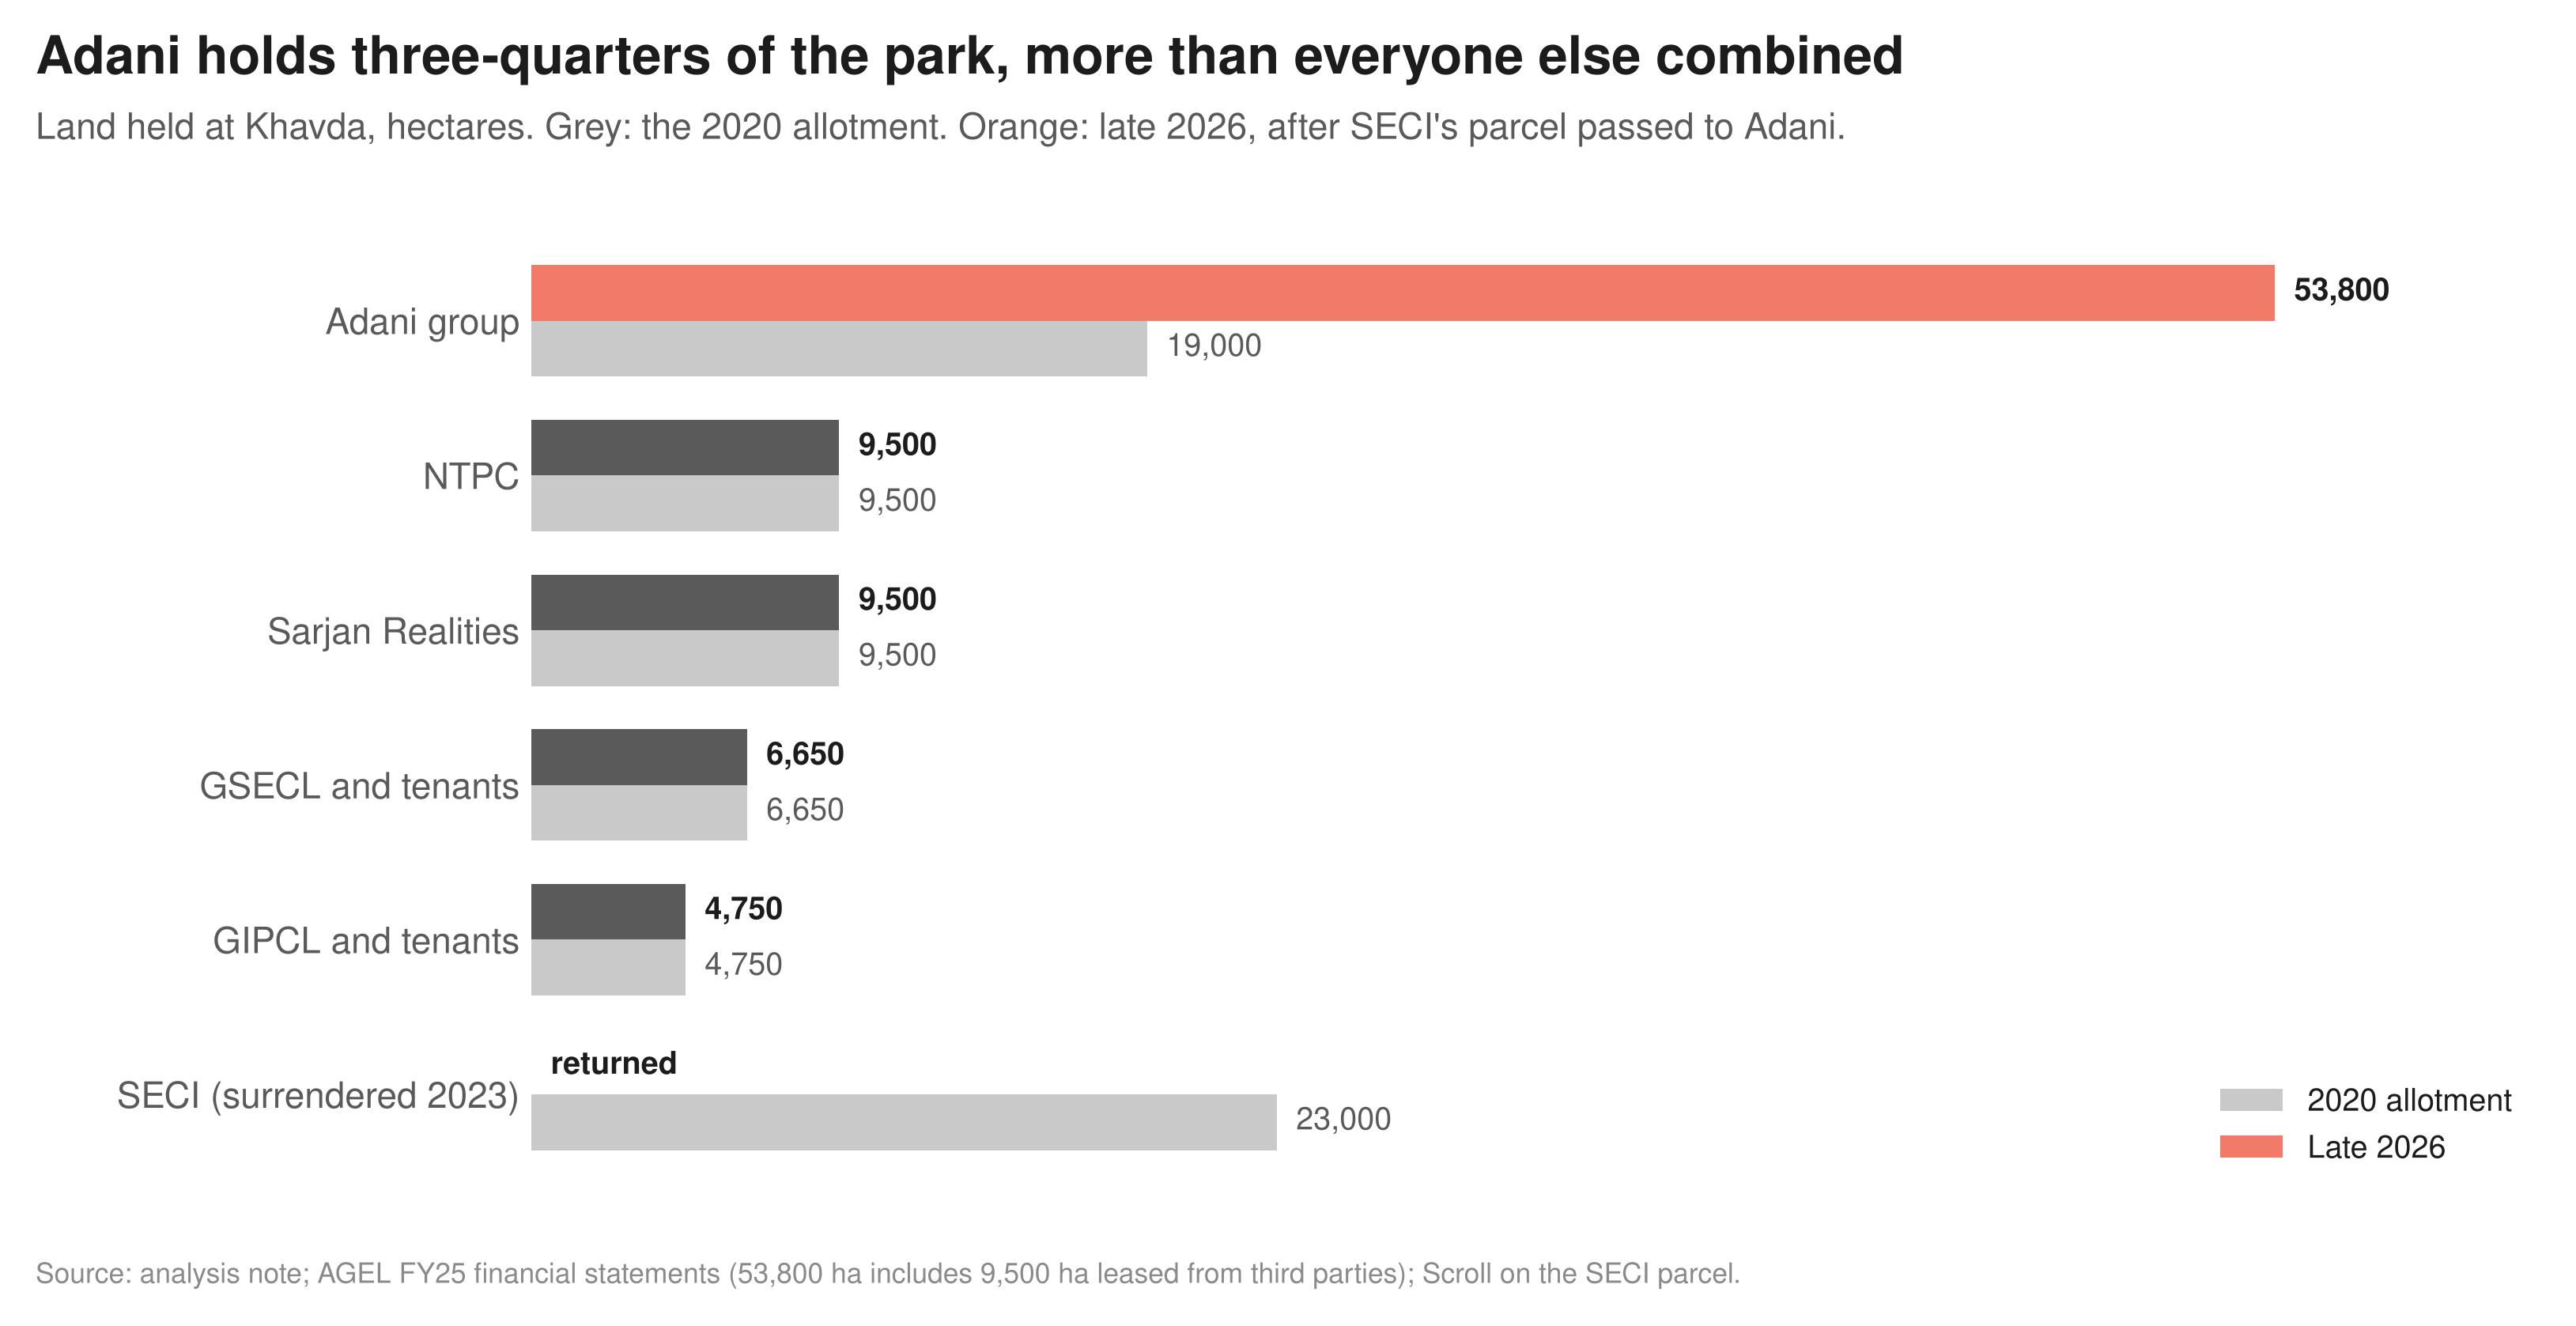
\includegraphics[width=\textwidth]{figures/fig_land_by_developer.png}
    \end{column}
    \begin{column}{0.5\textwidth}
      \satframe{\satLastFile}{\textwidth}{Latest frame with parcel outlines and hectares (needs \texttt{parcels.geojson} traced)}
      {\scriptsize\color{Ink2} Latest frame. Outlines and hectares from \texttt{parcels.geojson}; the orange trace is the measured built-up area.}
    \end{column}
  \end{columns}
  \note{Adani's holding came in two steps: 19,000 hectares in the 2020 allotment, the private cap, and the 23,000-hectare SECI parcel in 2023, after border rules changed and SECI gave it up. Plus 9,500 hectares leased from others. NTPC 9,500, Sarjan 9,500, GSECL 6,650, GIPCL 4,750.}
\end{frame}

% ==== 6. What the plant is made of ========================================
\begin{frame}{What the plant is made of}
  \begin{columns}[T]
    \begin{column}{0.6\textwidth}
      \begin{tikzpicture}[
          stage/.style={draw=Grey,fill=white,rounded corners=3pt,text width=7.4cm,
                        inner sep=4pt,font=\footnotesize,align=left},
          arr/.style={-{Stealth[length=2mm]},Grey,thick},
          node distance=2mm]
        \node[stage] (s1) {\textbf{1. Generate: panels and turbines}\\
          \scriptsize\color{Ink2} Bifacial panels on trackers, about 2,400 per MW. 5.2 MW turbines, 160 m rotor.};
        \node[stage,below=of s1] (s2) {\textbf{2. Convert and collect: inverters, 33 kV cables}\\
          \scriptsize\color{Ink2} Direct current to alternating; 1.36 MW of panels per MW of inverter. Cables underground, bedded in sand.};
        \node[stage,below=of s2] (s3) {\textbf{3. Pool: each developer's substations, 33 to 400 kV}\\
          \scriptsize\color{Ink2} Adani has 14, NTPC two, the others one or two each. Battery yards and voltage-support units sit beside them.};
        \node[stage,below=of s3,draw=SpOrange,fill=SpOrange!12] (s4) {\textbf{4. Export: Power Grid's stations, 400 to 765 kV}\\
          \scriptsize\color{Ink2} Three stations inside the park, KPS1 to KPS3. Two 765 kV lines out today; direct-current links from 2028.};
        \draw[arr] (s1) -- (s2); \draw[arr] (s2) -- (s3); \draw[arr] (s3) -- (s4);
      \end{tikzpicture}
    \end{column}
    \begin{column}{0.4\textwidth}
      \begin{tcolorbox}[colback=SpLightGray,colframe=SpLightGray,arc=3pt,left=3mm,right=3mm,top=1mm,bottom=1mm,boxsep=1mm]
        {\small\textbf{What must exist around it}}\\[2pt]
        {\scriptsize
        Roads raised 150 mm above flood level\\[1pt]
        Concrete mixed on site; Bhuj is 125 km\\[1pt]
        Water by tanker, rain tanks, desalting\\[1pt]
        Robots dry-clean panels most nights\\[1pt]
        Worker colonies with clinics on site\\[1pt]
        Own phone towers; one control room\\[1pt]
        Weather stations, fire station\\[1pt]
        Deep piles for salt, flood and quakes\\[1pt]
        Modules and turbines from Mundra\\[1pt]
        BSF permits; the border is 1 km away}
      \end{tcolorbox}
    \end{column}
  \end{columns}
  \note{Walk through the chain once, slowly. Panels make direct current; inverters make it alternating at 33 kV; each developer pools its feeders at its own 400 kV substation; Power Grid's three stations step it to 765 kV and send it out. Everything on the visit maps to one of these boxes.}
\end{frame}

% ==== 7. Building on salt =================================================
\begin{frame}{Building on salt}
  \vspace{1mm}
  \begin{columns}[T]
    \begin{column}{0.19\textwidth}\centering\midnum{45\% salt}{in the soil}\\[4pt]{\footnotesize Deep galvanised piles; cables bedded in sand}\end{column}
    \begin{column}{0.19\textwidth}\centering\midnum{3 m}{above sea level; floods in the monsoon}\\[4pt]{\footnotesize Roads raised 150 mm; inverters on plinths}\end{column}
    \begin{column}{0.19\textwidth}\centering\midnum{Zone V}{India's highest earthquake zone}\\[4pt]{\footnotesize Turbines on concrete rafts}\end{column}
    \begin{column}{0.19\textwidth}\centering\midnum{46°C}{summers; 50 to 70 dust storms a year}\\[4pt]{\footnotesize Robots clean panels dry, three nights a week}\end{column}
    \begin{column}{0.19\textwidth}\centering\midnum{No water}{the water table is hypersaline}\\[4pt]{\footnotesize Tankers, rain tanks, a desalination plant}\end{column}
  \end{columns}
  \vspace{2mm}
  \begin{tikzpicture}
    \node[fill=SpLightGray,draw=Grey,minimum width=\textwidth,minimum height=2.4cm,align=center,font=\small\color{Ink2}]
      {\textbf{Photo strip}: a pile being driven, a raised road, a cleaning robot, a worker colony.\\ No ground photographs in the package yet; drop them in \texttt{figures/photos/} and replace this box.};
  \end{tikzpicture}
  \note{The desert fights the plant. The answers are deep galvanised piles, roads raised 150 mm, cables bedded in sand, turbines on concrete rafts, robots that clean panels dry three nights a week, and colonies with clinics because nobody can commute from Bhuj.}
\end{frame}

% ==== 8. The timeline =====================================================
\begin{frame}{The timeline}
  \centering
  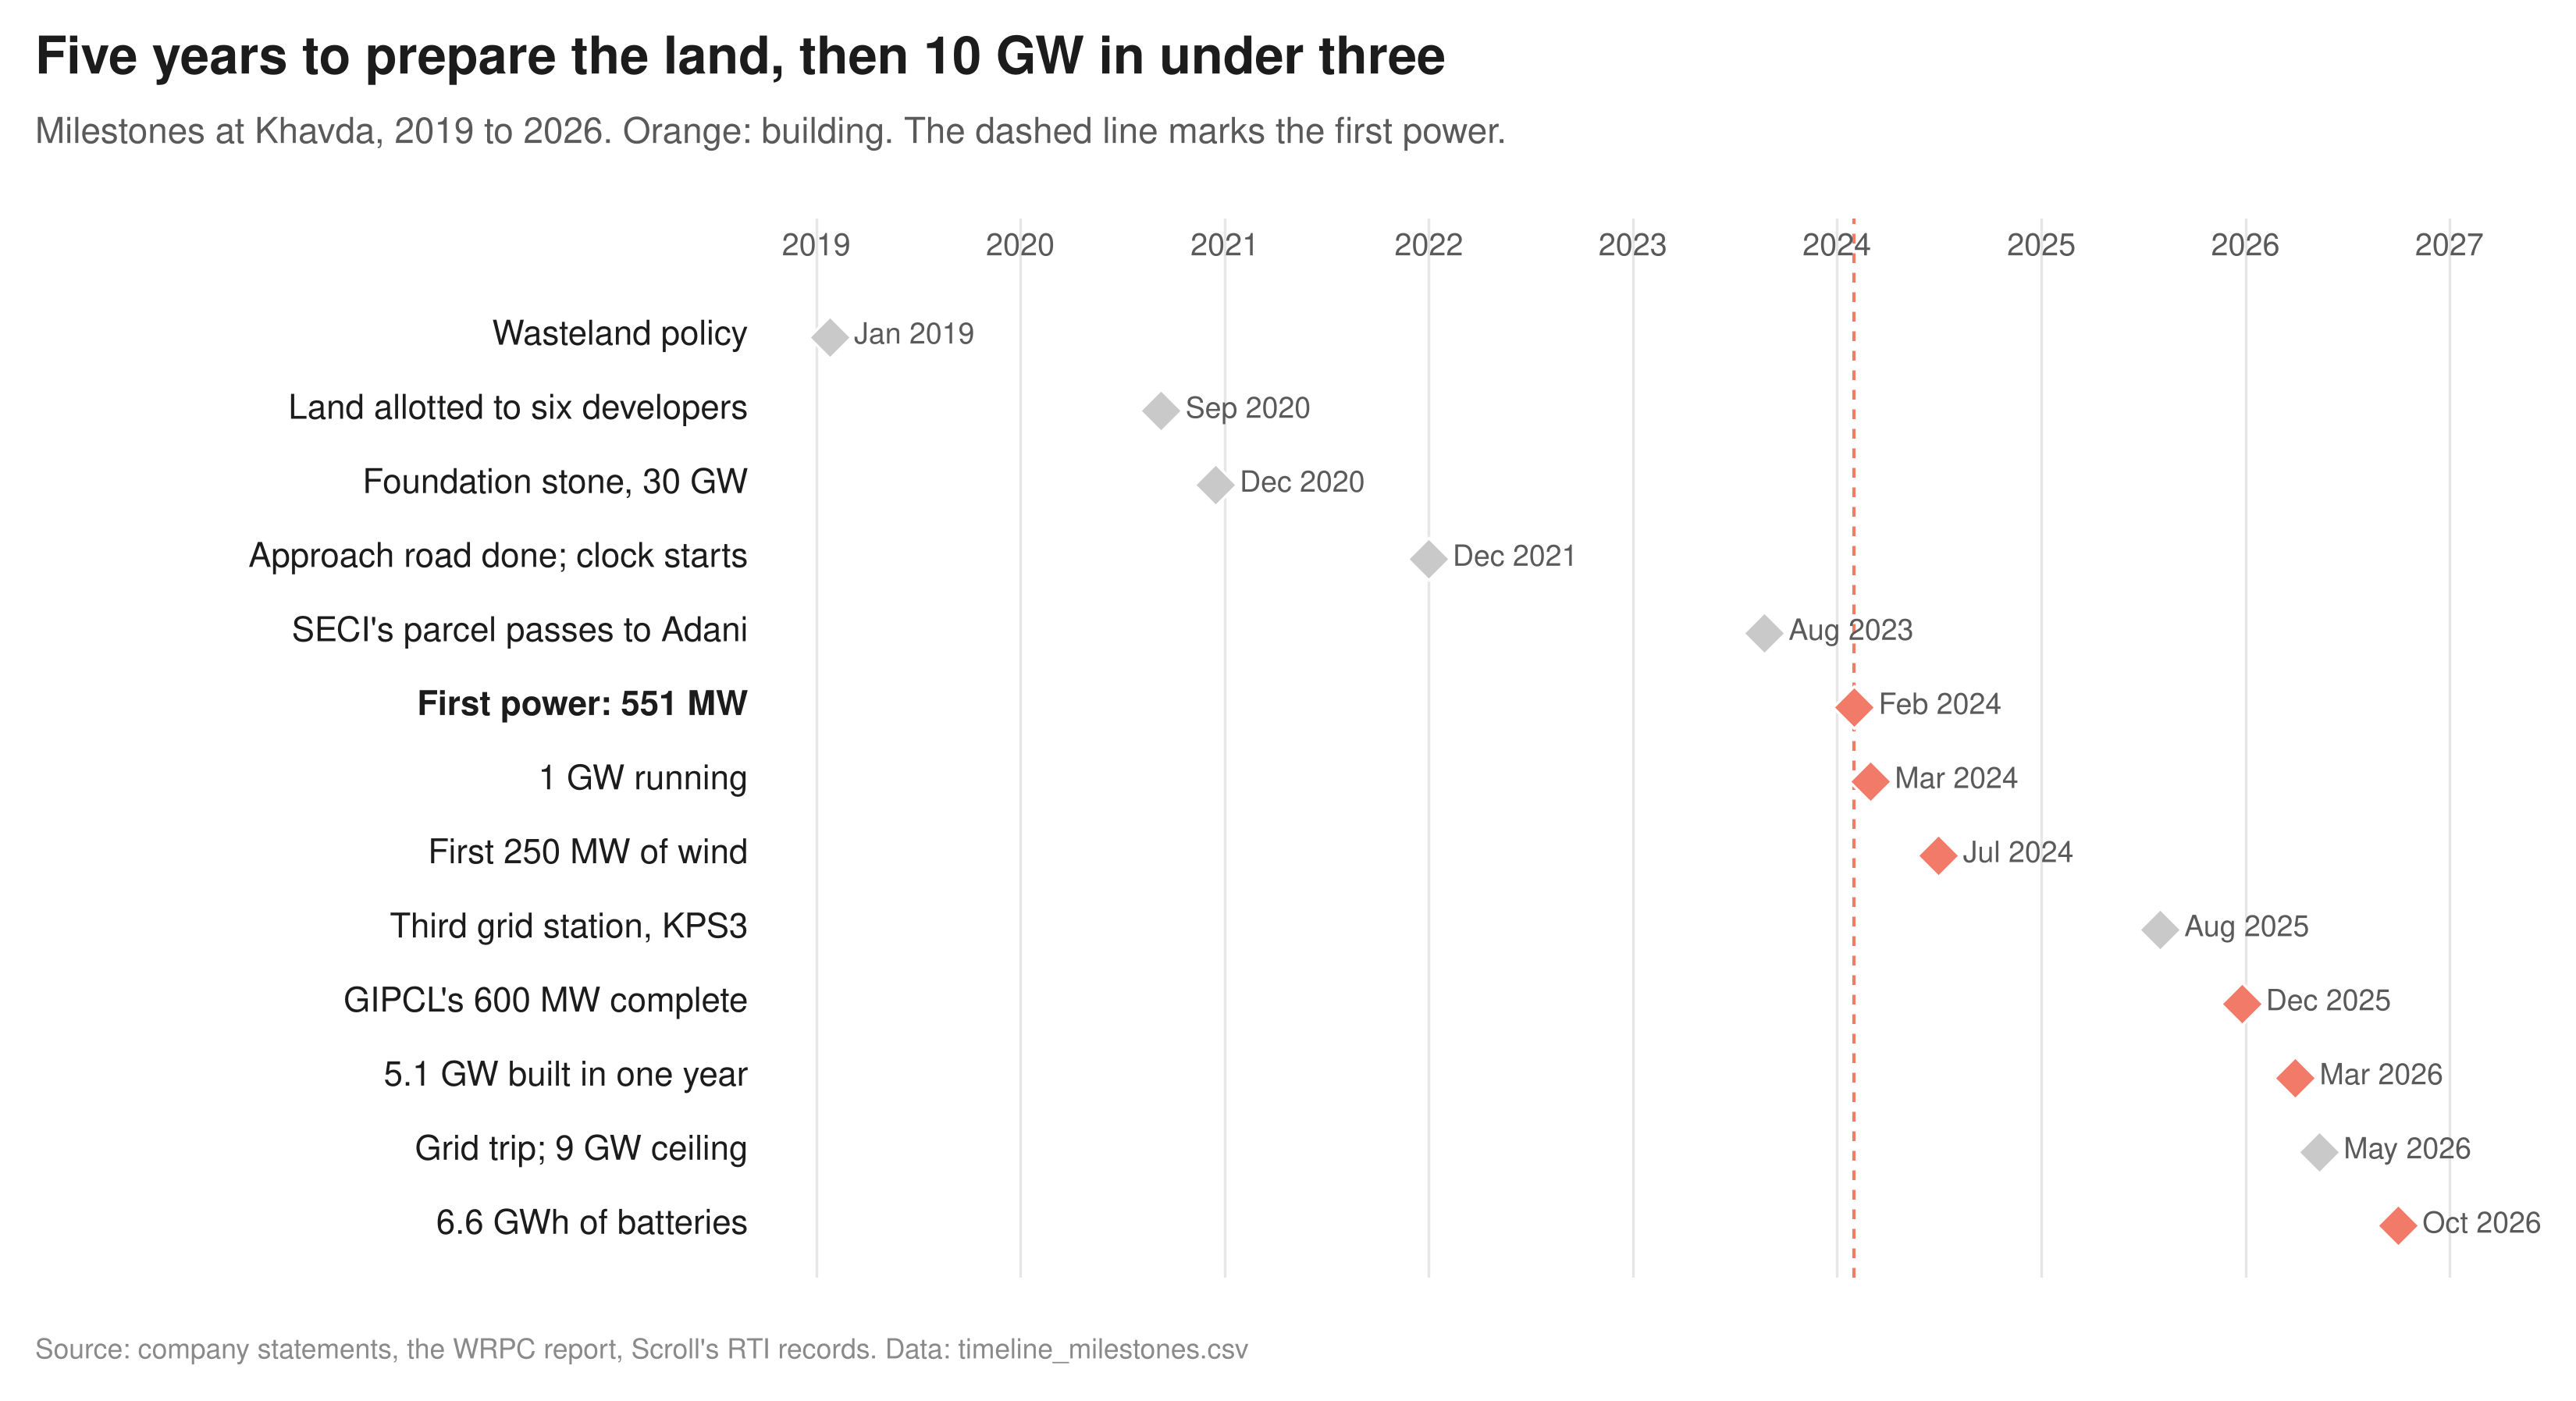
\includegraphics[width=0.83\textwidth]{figures/fig_timeline.png}
  \note{Three acts. Land, 2019 to 2023: policy, allotment, road, border deal. Build, 2024 to 2026: first power in February 2024, then 5 GW in one year. Wires, 2025 on: the stations and lines that lag the panels.}
\end{frame}

% ==== 9. CMIE =============================================================
\begin{frame}{What the CMIE capex data shows}
  \centering
  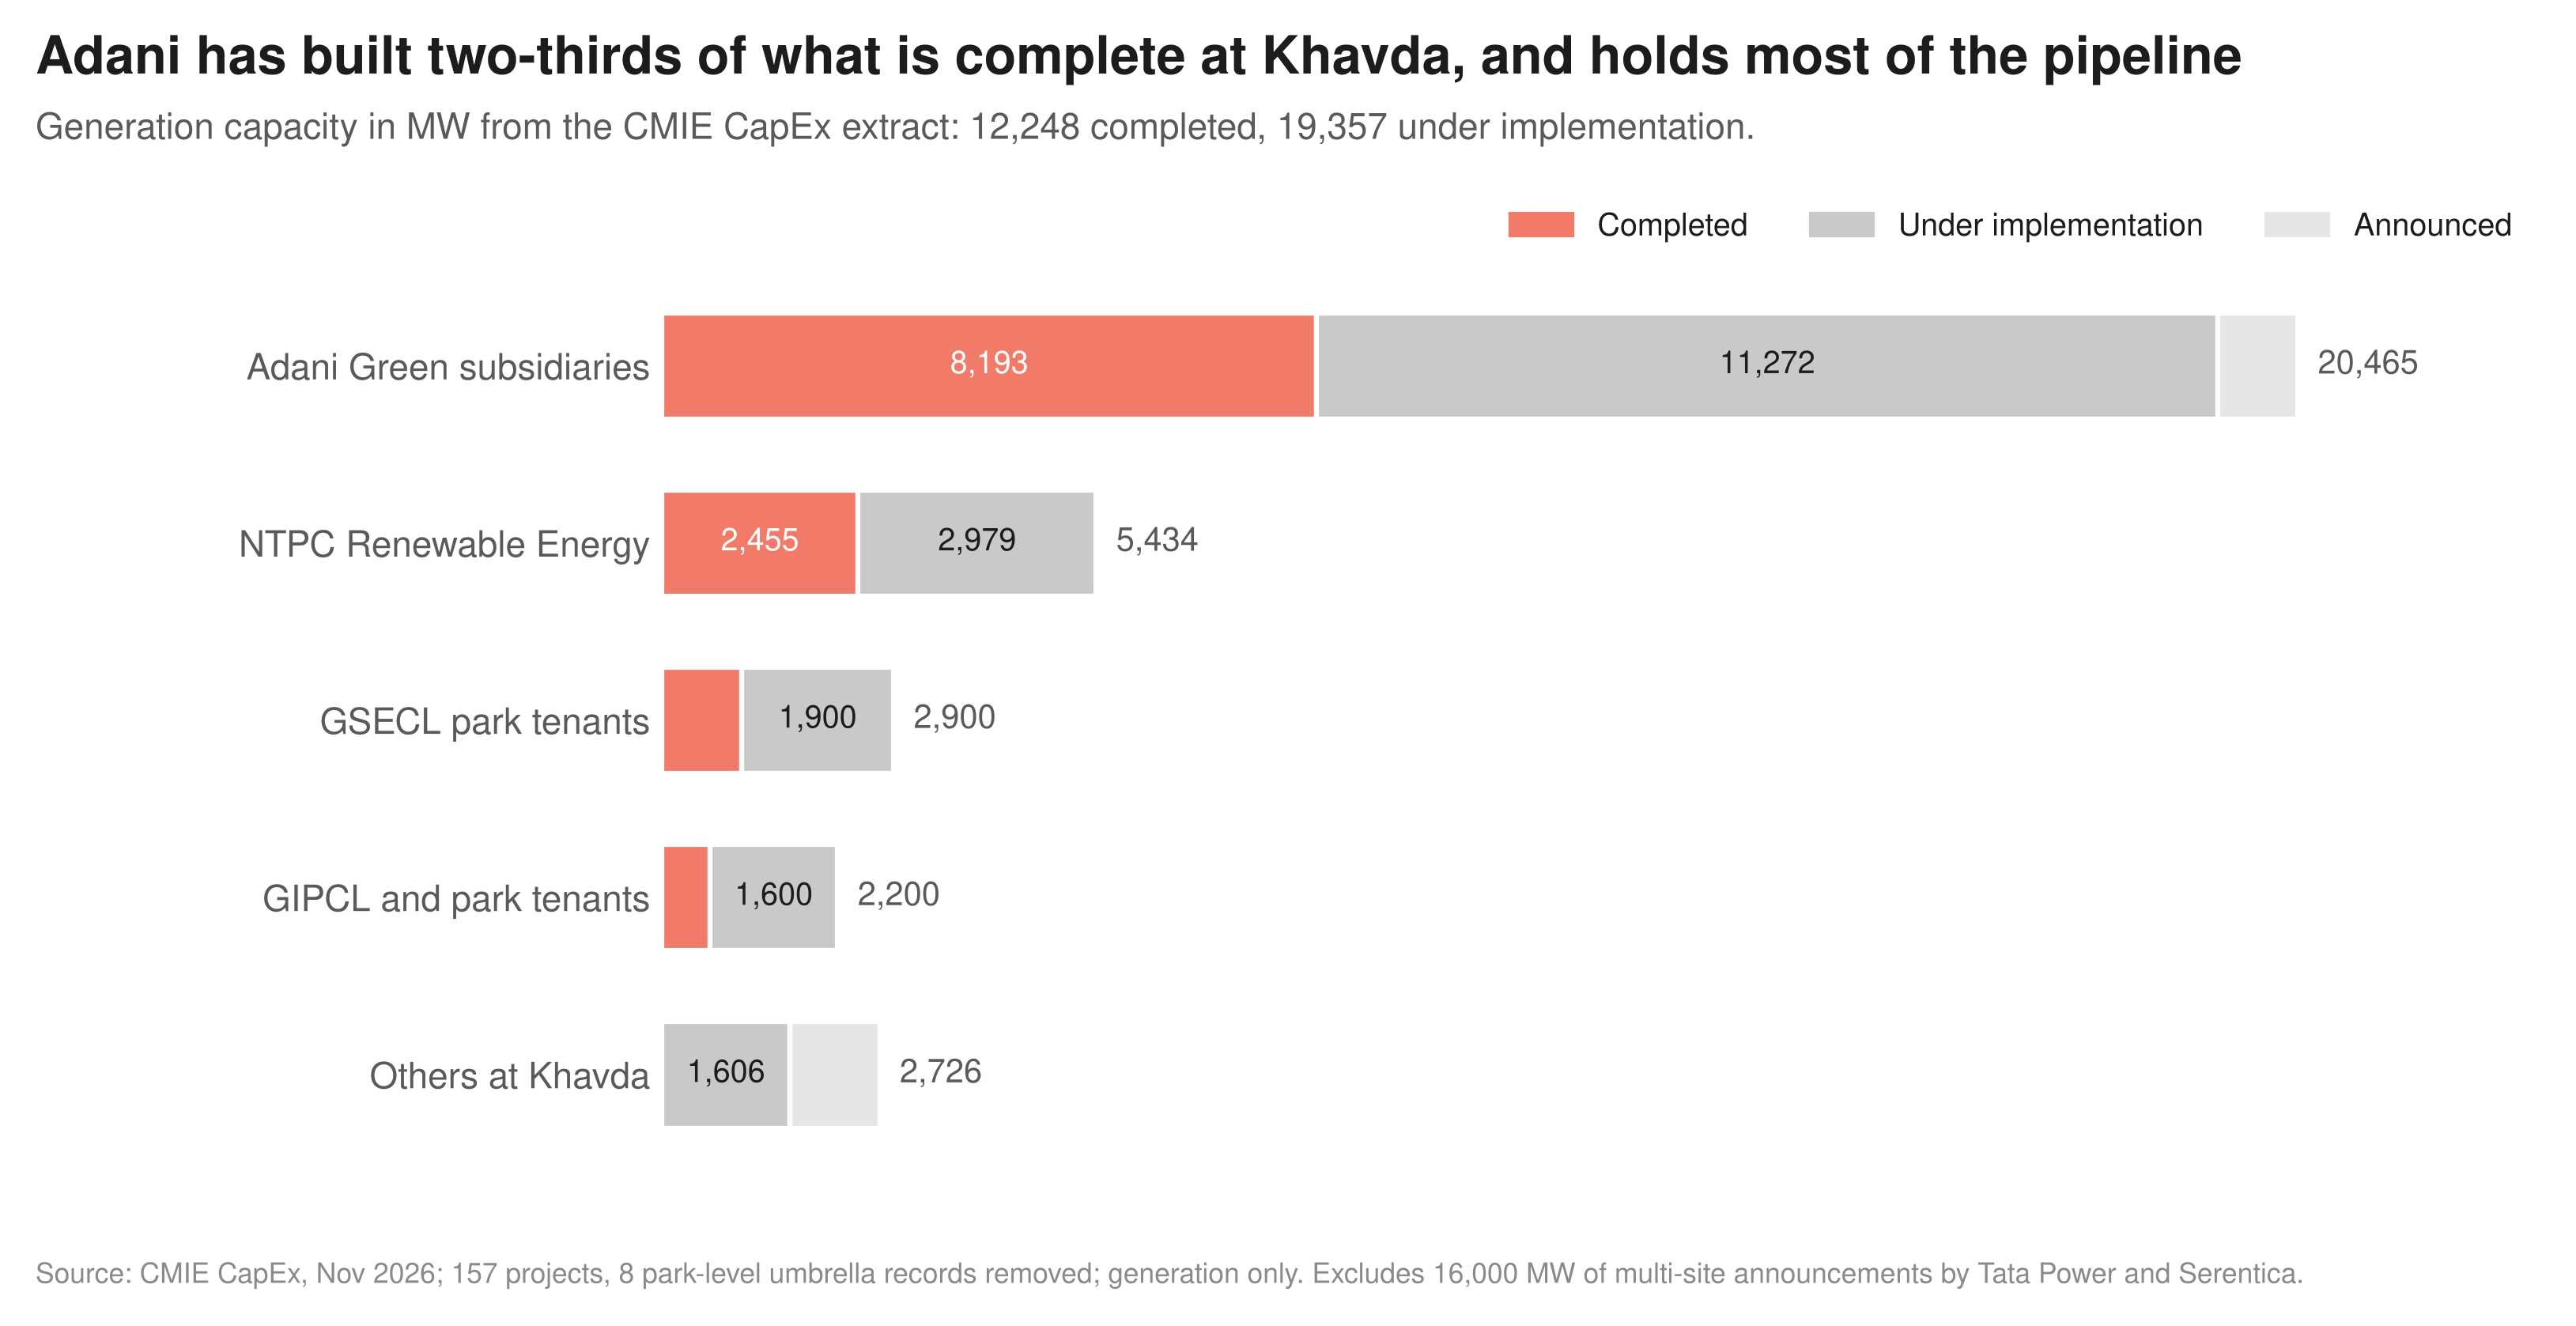
\includegraphics[width=0.9\textwidth]{figures/fig_capacity_by_developer.png}
  \note{CMIE tracks 157 projects at Khavda. It records the park twice, as umbrella entries and as plants, so the chart strips the umbrellas. 12 GW is done and 19 GW is under way; Adani has built two-thirds of the first and holds most of the second. NTPC is a distant second. The state landlords' tenants together have 1.6 GW running.}
\end{frame}

% ==== 10. How Adani builds ================================================
\begin{frame}{How Adani builds}
  \begin{columns}[T]
    \begin{column}{0.62\textwidth}
      \begin{tikzpicture}[
          box/.style={draw=Grey,fill=white,rounded corners=3pt,inner sep=5pt,font=\small,align=center},
          arr/.style={-{Stealth[length=2mm]},Grey,thick}]
        \node[box,text width=6.4cm,draw=SpOrange,fill=SpOrange!12] (agel)
          {\textbf{Adani Green Energy Ltd (AGEL)}\\ \footnotesize\color{Ink2} Listed. Owns the plants, raises the money};
        \node[box,text width=7.4cm,below=5mm of agel] (hold)
          {\textbf{Holding subsidiaries}\\ \footnotesize\color{Ink2} Bundle the plants so a partner such as TotalEnergies can buy a share};
        \node[box,text width=2.2cm,below=6mm of hold,xshift=-2.75cm] (a) {\textbf{AGE 24 Ltd}\\ \footnotesize\color{Ink2} 327 MW in 4 slices: 150, 100, 52, 25};
        \node[box,text width=2.2cm,below=6mm of hold] (b) {\textbf{AGE 25B Ltd}\\ \footnotesize\color{Ink2} 613 MW in 4 slices: 500, 83, 25, 5};
        \node[box,text width=2.2cm,below=6mm of hold,xshift=2.75cm] (c) {\textbf{AGE 27C Ltd}\\ \footnotesize\color{Ink2} 1,355 MWh battery, one of four};
        \draw[arr] (agel) -- (hold);
        \draw[arr] (hold.south) -- ++(0,-3mm) -| (a);
        \draw[arr] (hold.south) -- (b);
        \draw[arr] (hold.south) -- ++(0,-3mm) -| (c);
        \node[below=2mm of b,font=\scriptsize\color{Ink2},text width=7.6cm,align=center]
          {Three of 24 numbered subsidiaries in the CMIE sheet. Each signs its own contract and borrows on its own. Plants are declared complete in slices as small as 12.5 MW.};
      \end{tikzpicture}
    \end{column}
    \begin{column}{0.38\textwidth}
      \begin{tcolorbox}[colback=SpLightGray,colframe=SpLightGray,arc=3pt,left=3mm,right=3mm,top=1mm,bottom=1mm,boxsep=1mm]
        {\small\textbf{The group supplies every part}}\\[2pt]
        {\scriptsize
        \textbf{Adani New Industries}: panels and turbines, made at Mundra\\[2pt]
        \textbf{Adani Ports}: brings in the kit\\[2pt]
        \textbf{Ambuja and ACC}: the cement\\[2pt]
        \textbf{Adani Energy Solutions}: builds the lines out, both DC links\\[2pt]
        \textbf{Adani Infra}: the contractor, even on NHPC's 600 MW\\[2pt]
        \color{Ink2} Most of each rupee stays in the group}
      \end{tcolorbox}
    \end{column}
  \end{columns}
  \note{Each subsidiary holds one tranche of plant with its own contract and debt. Plants are declared complete in slices as each inverter yard is energised. Panels and turbines come from Mundra, cement from Ambuja, and the lines out are built by the group's transmission arm.}
\end{frame}

% ==== 11. Everyone else ===================================================
\begin{frame}{Everyone else}
  \begin{columns}[T]
    \begin{column}{0.58\textwidth}
      {\scriptsize\renewcommand{\arraystretch}{0.95}
      \begin{tabular}{@{}llrr@{}}
        \toprule
        \textbf{Tenant} & \textbf{Park, status} & \textbf{MW} & \textbf{Rs cr/MW} \\
        \midrule
        SAEL Solar P4 and P5 & GSECL, completed & 800 & 6.5 \\
        KPI Green Energy & GSECL, completed & 200 & 7.8 \\
        NLC India & GSECL, building & 600 & 5.6 \\
        SJVN Green (three plants) & GSECL, building & 600 & 4.3 to 5.5 \\
        JSW Renew Energy Ten & GSECL, building & 300 & -- \\
        NHPC & GSECL, building & 200 & 4.6 \\
        Enren-II Energy & GSECL, building & 200 & 6.5 \\
        GIPCL (own plant) & GIPCL, completed & 600 & 6.5 \\
        SJVN and SJVN Green & GIPCL, building & 700 & 5.4 to 6.5 \\
        SAEL Solar P6 & GIPCL, building & 400 & 3.25 \\
        Coal India & GIPCL, building & 300 & 6.5 \\
        NHPC & GIPCL, building & 200 & 4.1 \\
        \bottomrule
      \end{tabular}}
    \end{column}
    \begin{column}{0.4\textwidth}
      \begin{tcolorbox}[colback=SpLightGray,colframe=SpLightGray,arc=3pt,left=3mm,right=3mm,top=1mm,bottom=1mm,boxsep=1mm]
        \footnotesize
        \textbf{Two models side by side.} Adani and NTPC build their own plants. GSECL and GIPCL are landlords: they build substations and roads, then lease plots at 1.85 ha per MW to whoever wins a GUVNL auction.\\[4pt]
        \textbf{The tenants are the comparison group.} Same land, same rent, same technology, but bought at auction.\\[4pt]
        {\color{SpOrange}\textbf{CMIE records some at Rs 3.25 to 5.5 crore per MW against Adani's 6.5.}} Worth asking why on site.
      \end{tcolorbox}
    \end{column}
  \end{columns}
  \src{CMIE CapEx extract, Nov 2026. Costs are filed at announcement. NTPC, not shown: 2.5 GW done, builds its own.}
  \note{The tenants are the comparison group: same land, same rent, same technology, but bought at auction. CMIE records some of them at Rs 3.25 to 5.5 crore per MW against Adani's Rs 6.5. Worth asking why on site.}
\end{frame}

% ==== 12. Getting the power out ===========================================
\begin{frame}{Getting the power out}
  \centering
  \begin{tikzpicture}[
      box/.style={draw=Grey,fill=white,rounded corners=3pt,inner sep=4pt,font=\footnotesize,align=center,text width=2.3cm},
      kps/.style={box,text width=2.6cm},
      arr/.style={-{Stealth[length=2mm]},Grey,thick}]
    \node[box] (pan) {\textbf{Panels, turbines}\\ \footnotesize\color{Ink2} 33 kV collector lines};
    \node[box,right=4mm of pan,text width=2.5cm] (pool) {\textbf{Pooling substations}\\ \footnotesize\color{Ink2} 18 of them, 33 to 400 kV};
    \node[kps,right=6mm of pool,yshift=15mm] (k1) {\textbf{KPS1}\\ \footnotesize\color{Ink2} Adani only\\ 8,369 MW connected};
    \node[kps,right=6mm of pool] (k2) {\textbf{KPS2}\\ \footnotesize\color{Ink2} NTPC, GSECL, GIPCL\\ 3,155 MW connected};
    \node[kps,right=6mm of pool,yshift=-15mm] (k3) {\textbf{KPS3}\\ \footnotesize\color{Ink2} Adani, NTPC, Sarjan\\ 4,383 MW connected};
    \node[box,right=6mm of k1,text width=3.6cm,draw=SpOrange,fill=SpOrange!12,yshift=-2mm] (out)
      {\textbf{Two 765 kV lines out}\\ \footnotesize\color{Ink2} KPS1 to Bhuj, 107 km\\ KPS2 to Lakadia, 170 km\\ \textbf{\color{SpNearBlack}Limit: 9,000 MW of 14,800}};
    \node[box,right=6mm of k3,text width=3.6cm,yshift=2mm] (next)
      {\textbf{Coming, 2026 to 2029}\\ \footnotesize\color{Ink2} 765 kV to Halvad, delayed\\ 6 GW HVDC to Nagpur\\ 2.5 GW HVDC to South Olpad\\ 765 kV to Mumbai and Pune};
    \draw[arr] (pan) -- (pool);
    \draw[arr] (pool.east) -- ++(4mm,0) |- (k1.west);
    \draw[arr] (pool) -- (k2);
    \draw[arr] (pool.east) -- ++(4mm,0) |- (k3.west);
    \draw[arr] (k1.east) -- (out.west |- k1.east);
    \draw[arr] (k2.east) -- ++(4mm,0) |- (out.west);
    \draw[arr] (k3.east) -- (next.west |- k3.east);
    \draw[Grey,thick,dashed] (k2) -- (k3) node[midway,right,font=\tiny\color{Ink2}] {765 kV link};
  \end{tikzpicture}

  {\footnotesize\textbf{Panels take a year; lines take three to five.} The park outran its wires, so the operator caps it at 9,000 MW. \textcolor{Muted}{\tiny Source: WRPC grid disturbance report, May 2026, connected MW by station.}}
  \note{Two 765 kV corridors leave the park today, so the operator caps it at 9,000 MW out of 14,800 connected. The Halvad line was blocked at 229 of 690 tower sites by landowners. The fix is Rs 60,000 crore of new lines, mostly two direct-current links to Nagpur and Surat, on four-year builds.}
\end{frame}

\begin{frame}{The corridors out of Kutch}
  \centering
  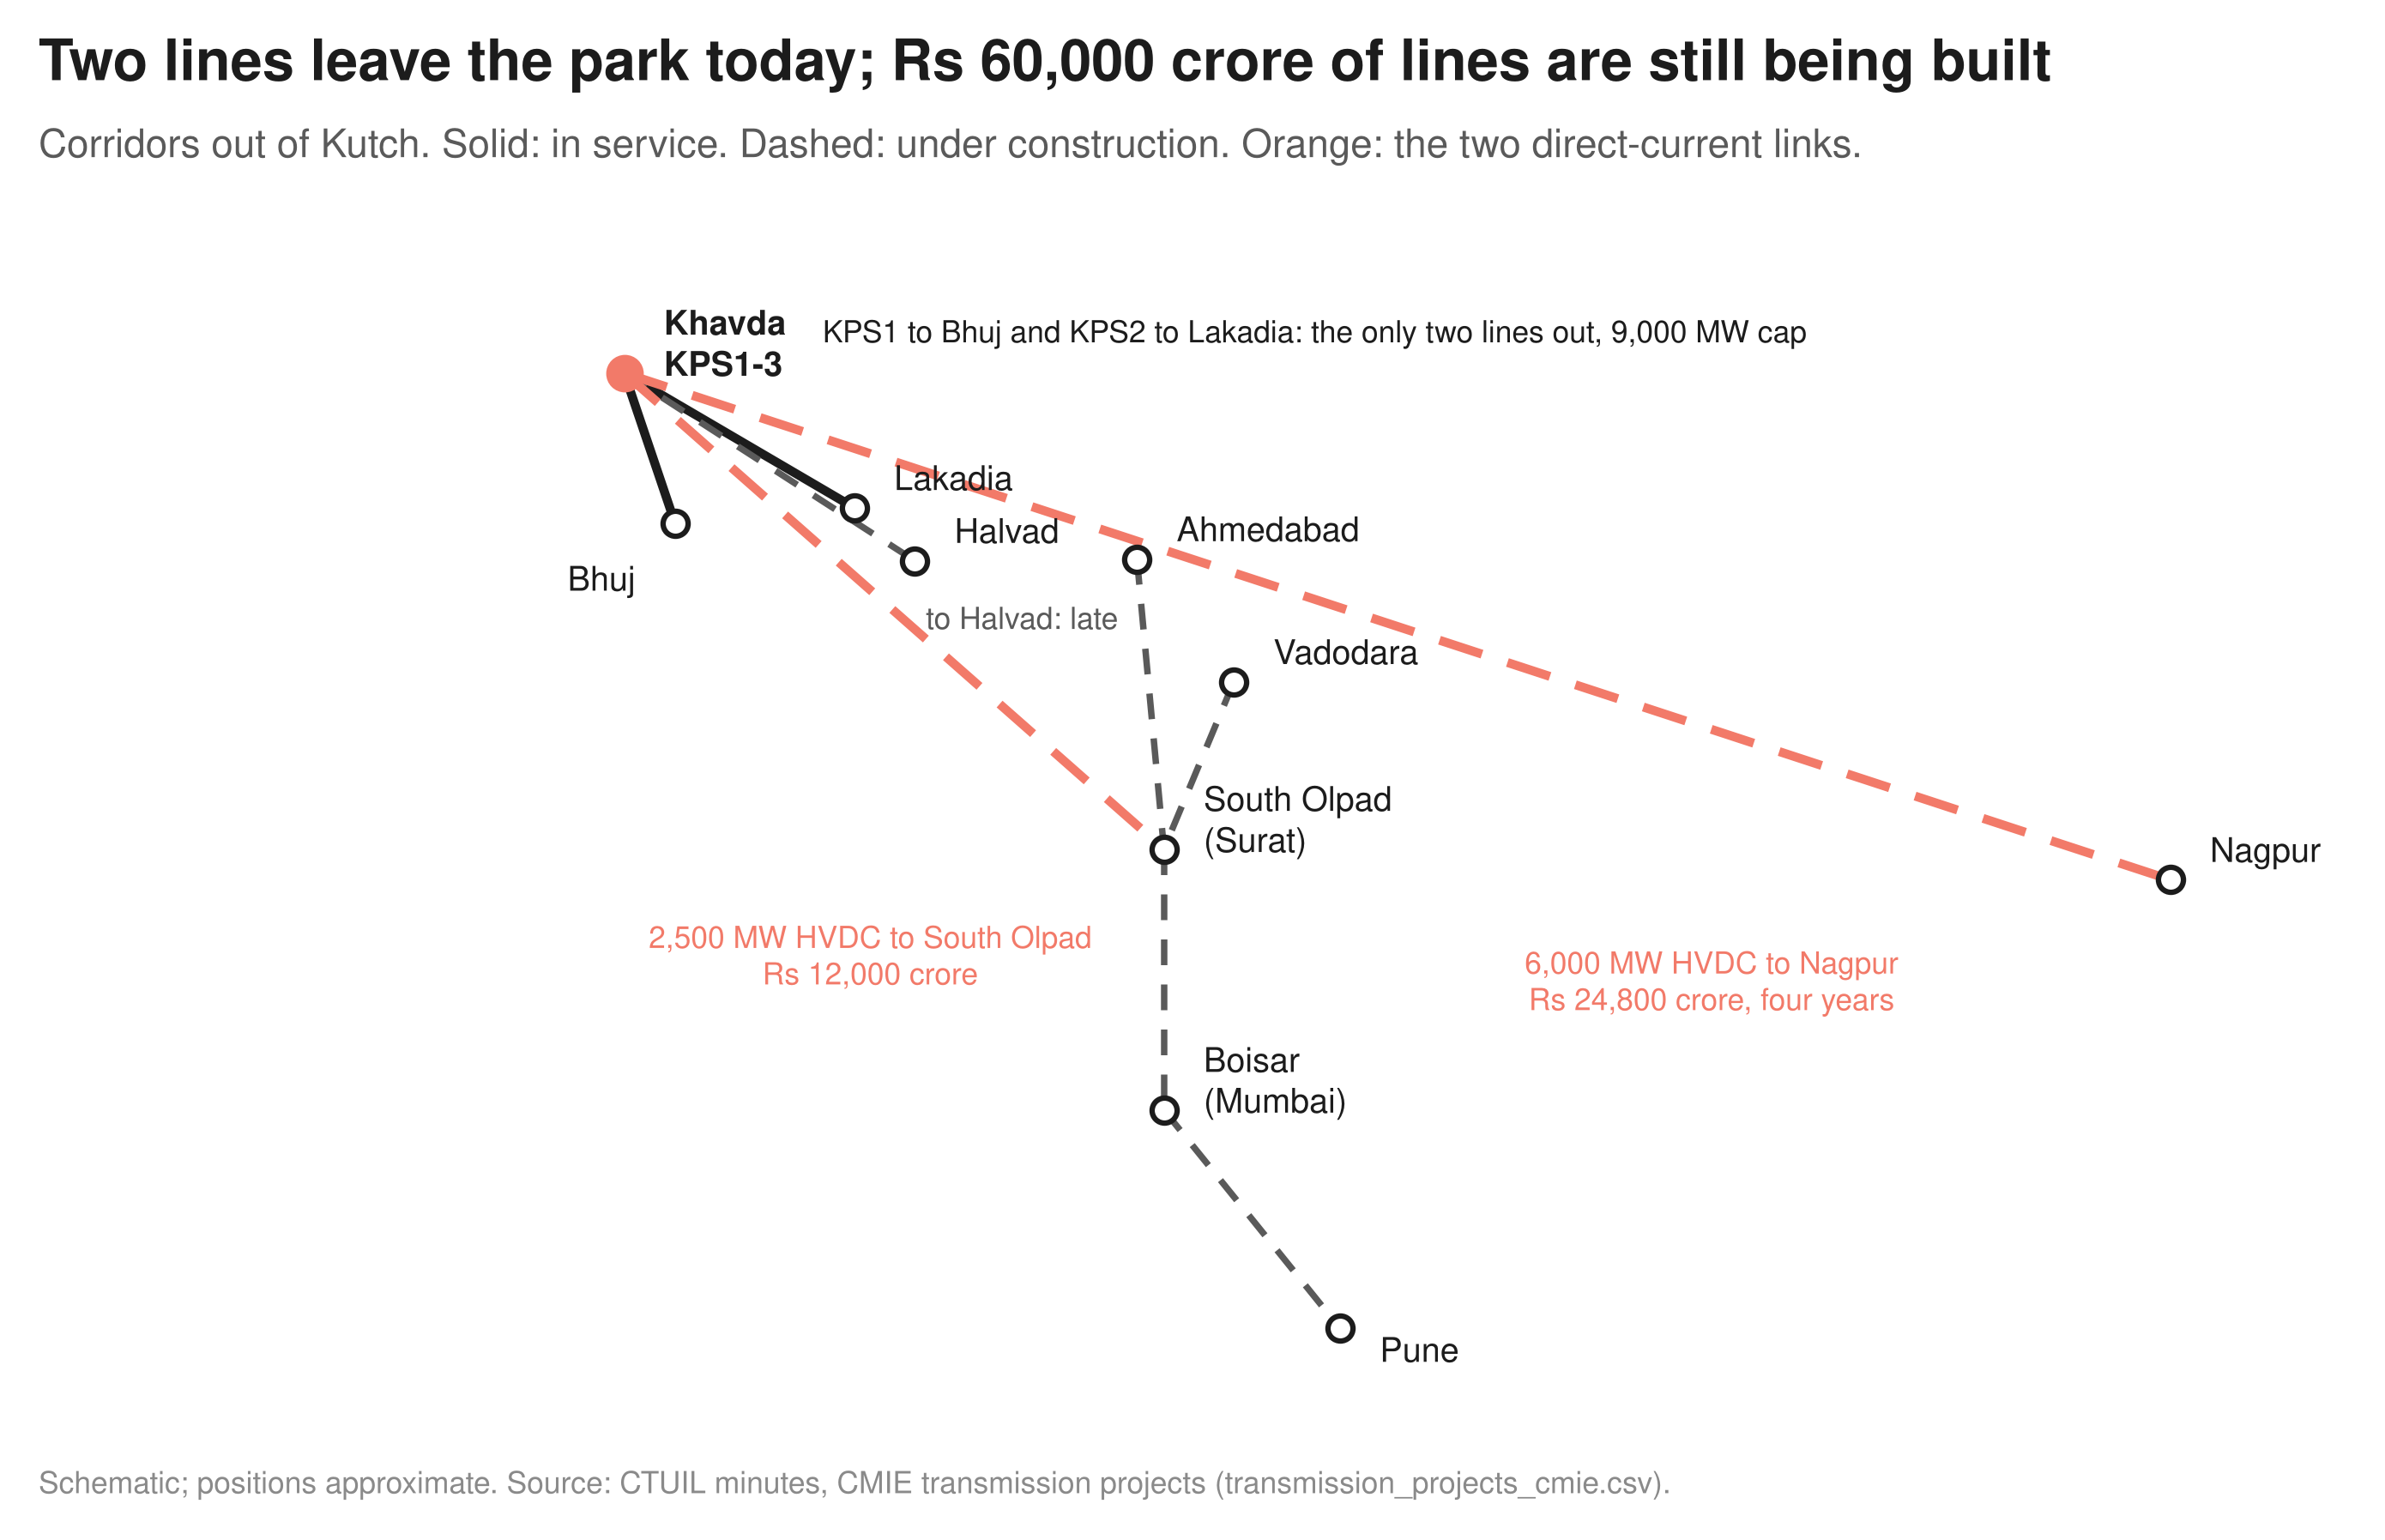
\includegraphics[width=0.72\textwidth]{figures/fig_corridors.png}
  \note{Phase III to Halvad: due December 2025, slipped into 2026; landowners blocked 229 of 690 tower sites and 267 hectares of forest clearance was pending. Phase IV south through South Olpad to Boisar and Pune. Phase V: the two direct-current links, four-year builds. The two DC links cost more than all the AC lines together.}
\end{frame}

% ==== 13. 13 May 2026 =====================================================
\begin{frame}{13 May 2026: dark in 17 seconds}
  \centering
  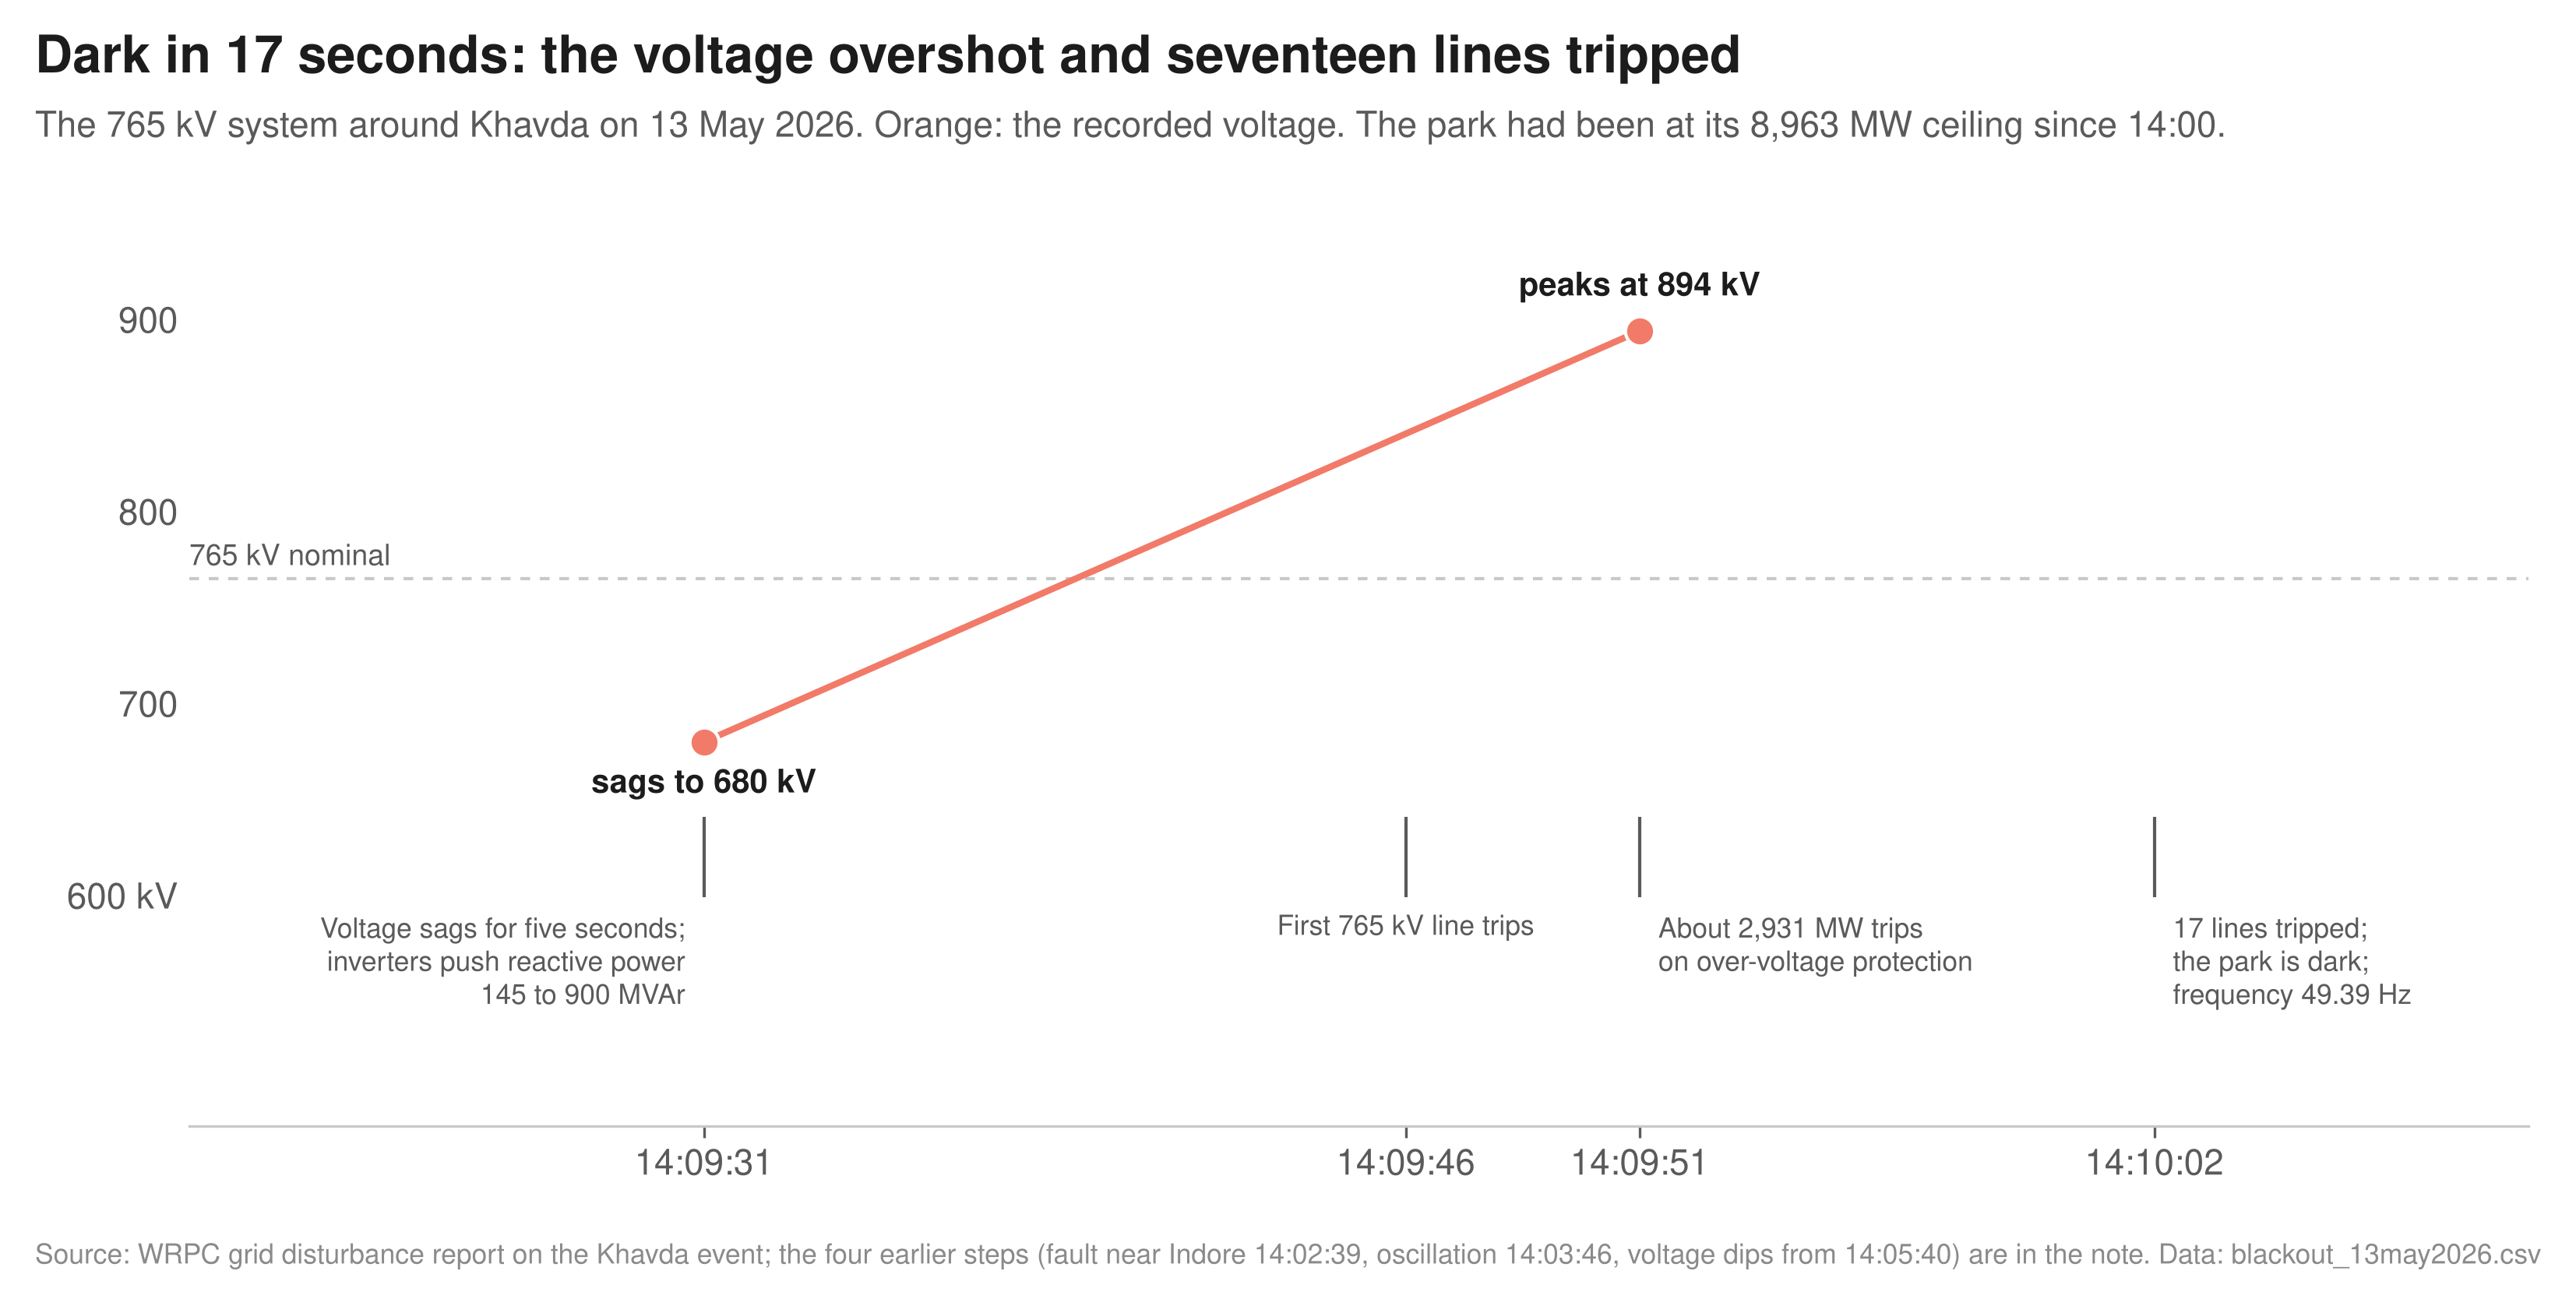
\includegraphics[width=0.88\textwidth]{figures/fig_blackout.png}
  \note{A distant fault made the inverters push reactive power to hold voltage up; a weak grid with no spinning generators could not absorb it; voltage overshot, plants tripped, lines unloaded, voltage rose further. Western India shed load. The fix is voltage-support units at the stations and a direct-current link that can hold voltage on its own.}
\end{frame}

% ==== 14. Batteries =======================================================
\begin{frame}{Batteries as the stopgap}
  \begin{columns}[T]
    \begin{column}{0.56\textwidth}
      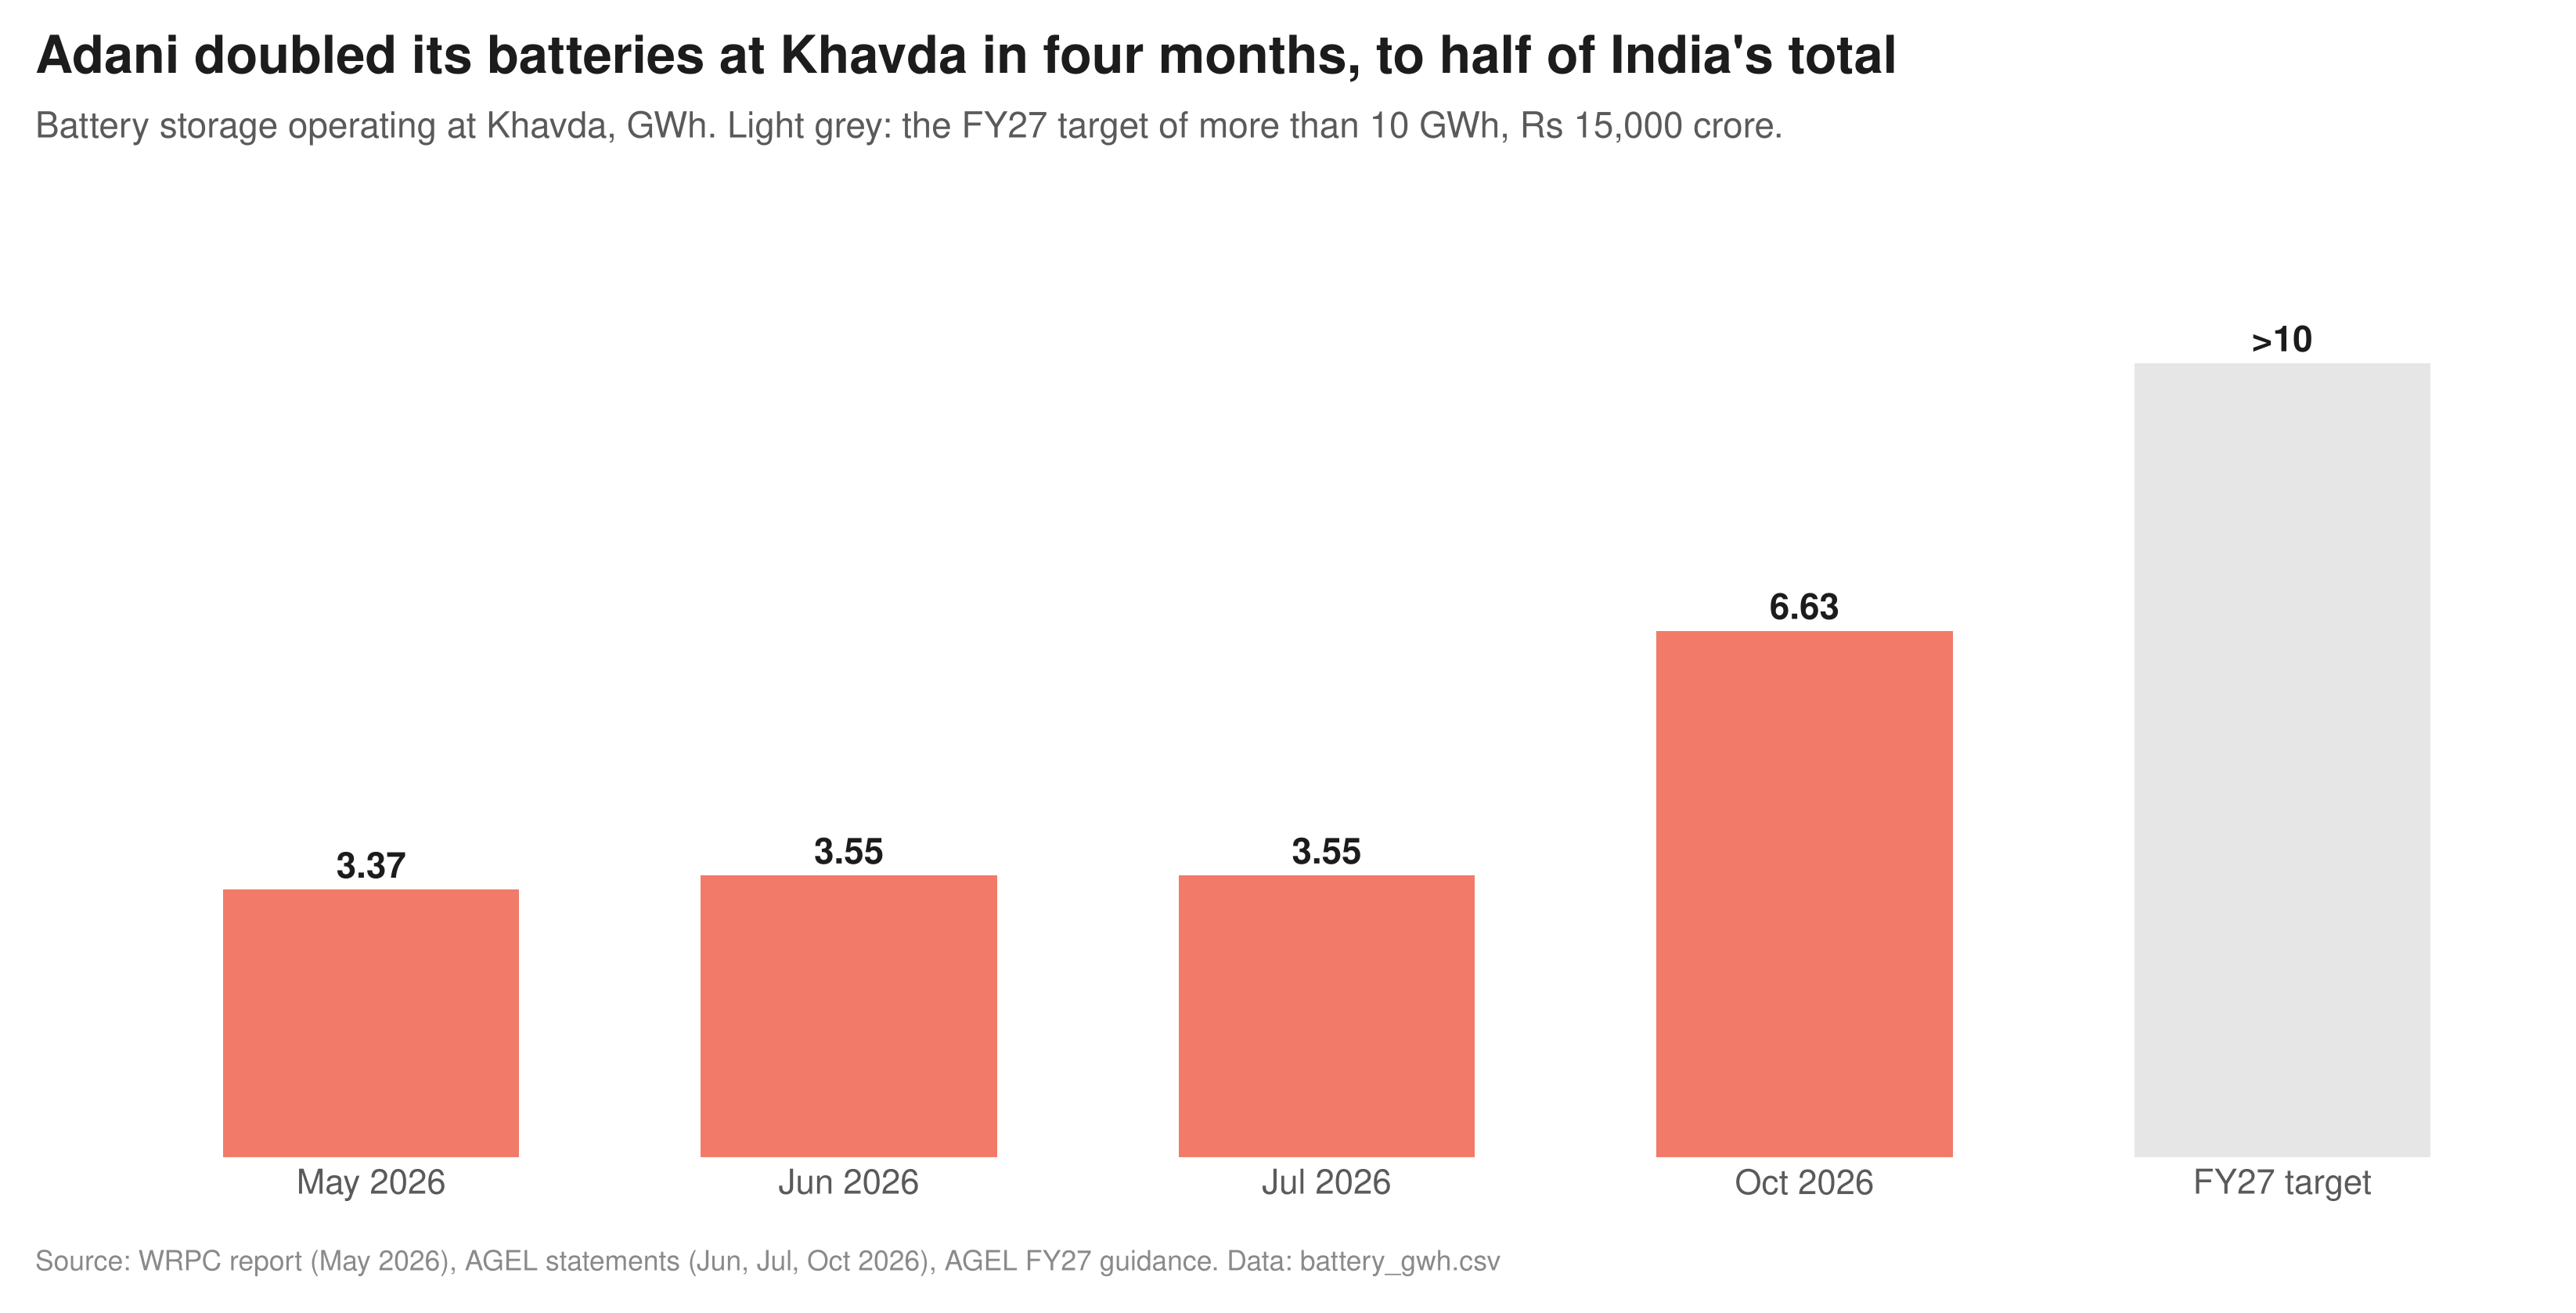
\includegraphics[width=\textwidth]{figures/fig_battery.png}
    \end{column}
    \begin{column}{0.44\textwidth}
      {\small\textbf{When the line is full at noon, power is lost.} Batteries store it and sell it at 7 pm.}\\[5pt]
      \midnum{6.6 GWh}{in October 2026, half of India's total}\\[5pt]
      \midnum{Rs 15,000 cr}{to pass 10 GWh in FY27}\\[5pt]
      {\footnotesize\color{Ink2} Curtailment could cost 5 to 7\% of group EBITDA until the lines open. On the satellite image the battery yards are the dense rectangles beside the switchyards.}
    \end{column}
  \end{columns}
  \note{Curtailment could cost Adani 5\% to 7\% of group earnings until the lines open. The battery yards sit beside the pooling substations; on the satellite image they are the dense rectangles next to the switchyards. To show them: circle them with a polygon in a second GeoJSON and render one still with --polygons.}
\end{frame}

% ==== 15. Economics =======================================================
\begin{frame}{The economics}
  \begin{columns}[T]
    \begin{column}{0.62\textwidth}
      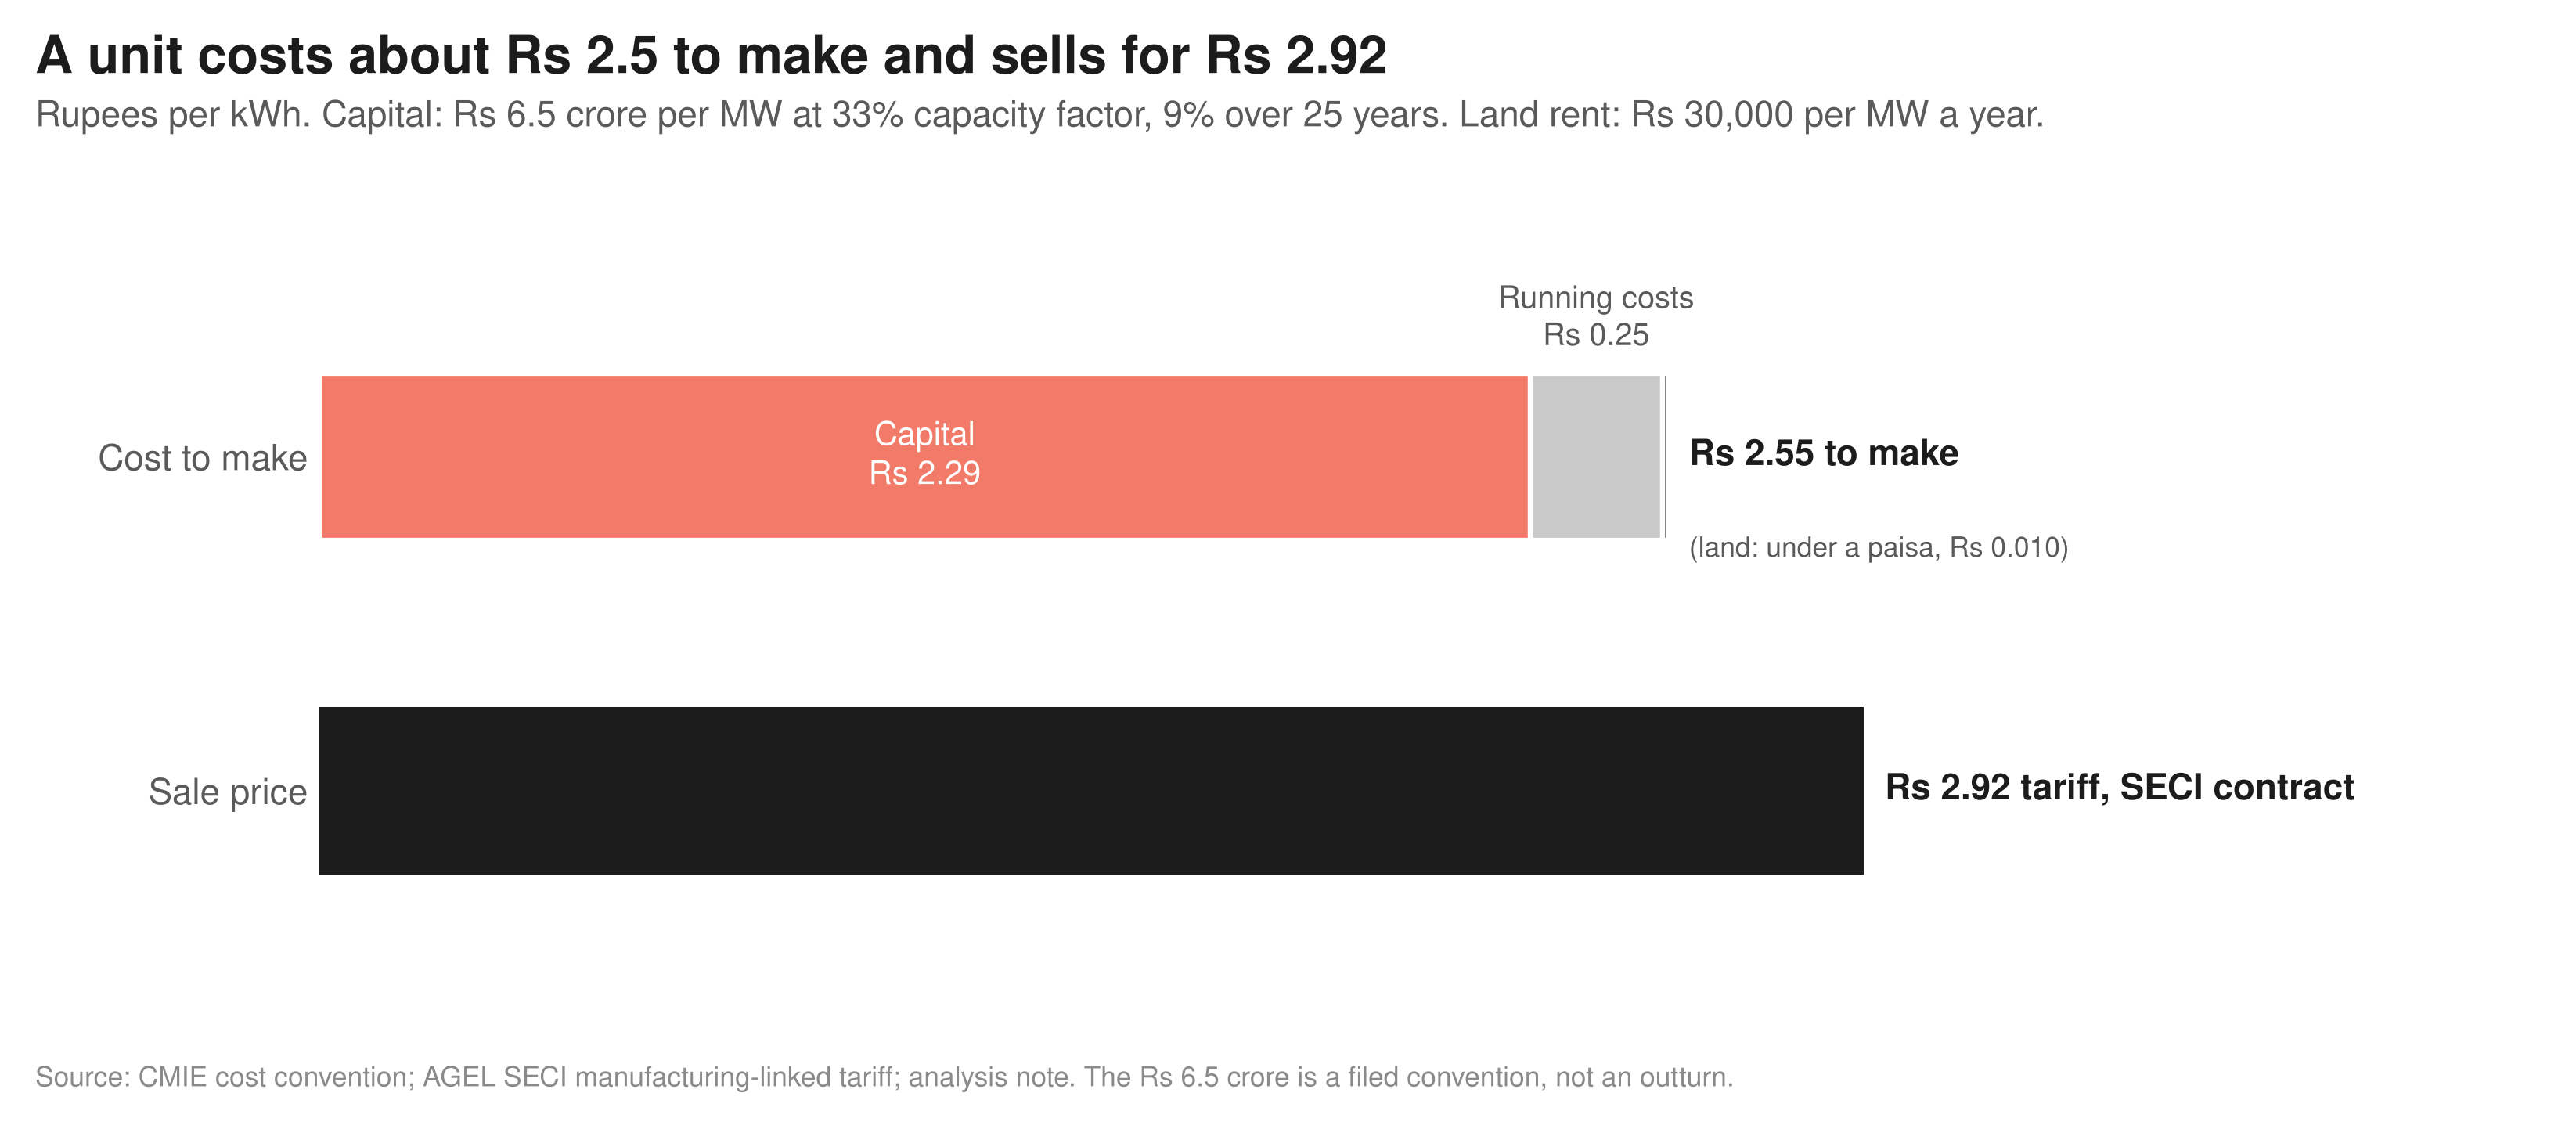
\includegraphics[width=\textwidth]{figures/fig_cost_stack.png}
    \end{column}
    \begin{column}{0.38\textwidth}
      \vspace{2mm}
      {\small
      \textbf{Who buys the power}\\[3pt]
      25-year contracts with SECI, NTPC and GUVNL.\\[3pt]
      Corporates: Google (Oct 2024), Asahi India Glass (Jan 2026).\\[3pt]
      The evening exchange market, for battery power.\\[8pt]
      \textbf{When finished}\\[3pt]
      81 to 87 billion units a year: about 4\% of what India uses.}
    \end{column}
  \end{columns}
  \note{The Rs 6.5 crore is CMIE's convention, filed at announcement. The real number, and what it includes, is a question for the visit. The margin is real but thin, and it depends on the 33\% being achieved and the power being carried away.}
\end{frame}

% ==== 16. Adani in four points ============================================
\begin{frame}{Adani, in four points}
  \vspace{1mm}
  \begin{enumerate}\setlength{\itemsep}{6pt}
    \item Got the private cap of land, 19,000 ha, in 2020, and the 23,000 ha SECI parcel in 2023 without a tender.
    \item Faced a US indictment in November 2024 over the SECI contracts; dropped and settled in 2026 with no admission.
    \item Built 5.1 GW at Khavda in the year that straddled it.
    \item Its own transmission arm builds the lines out, including both direct-current links.
  \end{enumerate}
  \vspace{3mm}
  \begin{tcolorbox}[colback=SpLightGray,colframe=SpLightGray,arc=2pt,left=4mm,right=4mm,top=1mm,bottom=1mm]
    \small Neither the share-price shock of 2023 nor the indictment of 2024 slowed the build. The slow lines cost one Adani company, AGEL, lost power, and pay another, Adani Energy Solutions, to build them.
  \end{tcolorbox}
  \note{Keep this short. The point for the audience is that neither episode slowed the build.}
\end{frame}

% ==== 17. The plant in one page ===========================================
\begin{frame}{The plant in one page}
  \begin{columns}[T]
    \begin{column}{0.5\textwidth}
      \begin{tcolorbox}[colback=SpOrange!12,colframe=SpOrange,arc=3pt,left=3mm,right=3mm,top=0.5mm,bottom=0.5mm,boxsep=1mm]\small
        \textbf{Inside the park: fast.} One owner, flat land, factory kit, 5 GW a year.
      \end{tcolorbox}
      \begin{tcolorbox}[colback=SpLightGray,colframe=Grey,arc=3pt,left=3mm,right=3mm,top=0.5mm,bottom=0.5mm,boxsep=1mm]\small
        \textbf{Outside: slow.} Farmland, forests, three to five years a line.
      \end{tcolorbox}
      \begin{tcolorbox}[colback=white,colframe=Grey,arc=3pt,left=3mm,right=3mm,top=0.5mm,bottom=0.5mm,boxsep=1mm]\small
        \textbf{Between: batteries.} 9 GW cap, lost noon power, 6.6 GWh of storage.
      \end{tcolorbox}
      {\footnotesize\color{Ink2} The question for the visit: when the lines open in 2027 to 2029, does the thin margin hold, and does the landlord-tenant model prove cheaper than Adani's own?}
    \end{column}
    \begin{column}{0.5\textwidth}
      \satframe{\satLastFile}{\textwidth}{Latest frame, annotated: the three KPS stations and the two lines out}
      {\scriptsize\color{Ink2} Latest frame. Mark KPS1 to KPS3 and the two corridors as polygons in \texttt{parcels.geojson}.}
    \end{column}
  \end{columns}
  \note{Close on the question the visit should answer.}
\end{frame}

% ==== 18. Build-out curve (after make_frames.sh) ==========================
\begin{frame}{What the frames measure}
  \centering
  \satframe{figures/fig_buildout_curve.png}{0.8\textwidth}{Built-up hectares per quarter, measured from the frames, against the milestones. Appears after \texttt{make\_frames.sh} then \texttt{make\_figures.py}.}
  \note{The orange outline in the animation is a luminance cut: dark ground that was not dark in 2020 and stays dark to the end. At two hectares per MW it gives an independent MW estimate to set against the announced figures. Monsoon quarters are the least reliable.}
\end{frame}

% ==== 19. Sources =========================================================
\begin{frame}{Sources}
  {\scriptsize
  \begin{itemize}\setlength{\itemsep}{2pt}
    \item WRPC, grid disturbance report on Khavda, 13 May 2026: connected capacity by station, the 9,000 MW limit, the second-by-second record.
    \item CTUIL, minutes on evacuation beyond 15 GW (19 Dec 2022) and 37th CMETS-WR minutes: transmission phases, the Halvad delay.
    \item AGEL, the 30 GW Khavda project page; AGEL ESIA for the 9,500 MW hybrid projects; AGEL FY25 consolidated financial statements.
    \item ADB, SAEL Gujarat solar project IEE: the GSECL sub-park model, 1.85 ha per MW.
    \item Scroll, how Adani bagged the border project: the 2023 sequence from RTI records.
    \item CMIE CapEx extract, Nov 2026: 260 rows, 157 projects at Khavda; umbrella records removed.
    \item ET Energy, DSIJ, Indian Infrastructure, Saur Energy, India TV, FilingReader, GIPCL, KPI Green annual report FY26: dated commissioning and corporate events.
    \item Satellite imagery: Copernicus Sentinel-2 (COPERNICUS/S2\_SR\_HARMONIZED) via Google Earth Engine; contains modified Copernicus Sentinel data. Built-up area is a luminance threshold, not a land-cover classification.
  \end{itemize}
  \vspace{3mm}
  \color{Ink2} India's annual generation is quoted from memory and is approximate; everything else traces to the files or pages above.}
\end{frame}

\end{document}
